\documentclass{article}

\usepackage{geometry}
\geometry{hmargin = 4cm, vmargin = 2cm}

\usepackage{amsthm}
\newtheorem{proposition}{Proposition}[section]
\theoremstyle{definition}
\newtheorem{definition}{Definition}[section]
\newtheorem{theorem}{Theorem}[section]
\newtheorem{example}{Example}[section]
\theoremstyle{remark}
\newtheorem{remark}{Remark}[section]
\newtheorem{lemma}{Lemma}[section]

\setlength{\parskip}{0.5em}

\usepackage{multicol}
\usepackage[linesnumbered,ruled,vlined]{algorithm2e}
\usepackage{comment}
\usepackage{pgf}
\usepackage{tikz}
\usetikzlibrary{arrows,automata}
\usepackage[utf8]{inputenc} 		% encodage des caracteres utilise (pour les caracteres accentues) -- non utilise ici.
%\usepackage[latin1]{inputenc} 		% autre encodage
\usepackage[english]{babel}		% pour une mise en forme "anglaise"
\usepackage{amsmath,amssymb,amsthm}	% pour les maths
\usepackage{graphicx}			% pour inclure des graphiques
\usepackage{hyperref}			% si vous souhaitez que les references soient des hyperliens
\usepackage{color}			% pour ajouter des couleurs dans vos textes
\usepackage{todonotes}

\def \N {\mathbb N}	

\newcommand{\TodoDavid}[1]{\todo[color=green!40]{#1}}
\newcommand{\TodoJF}[1]{\todo{#1}}

\newcommand{\tr}{\textit{tr}}
\newcommand{\Vars}{\textbf{Vars}}
\newcommand{\MC}{\textbf{MC}}
\newcommand{\Terms}{\textbf{Terms}}
\newcommand{\Preds}{\textbf{Preds}}
\newcommand{\Csts}{\textbf{Csts}}
\newcommand{\Merge}{\textit{Merge}}
\newcommand{\Depth}{\textit{depth}}
\newcommand{\Appl}{\textbf{appl}}
\newcommand{\father}{\textbf{father}}
\newcommand{\Tree}{\textit{Tree}}
\newcommand{\Fut}{\textbf{Fut}}
\newcommand{\des}{\textbf{Desc}}
\newcommand{\ALCH}{\textbf{Horn-$\mathcal{ALCH}$}}
\newcommand{\ALCHI}{\textbf{Horn-$\mathcal{ALCHI}$}}

\title{Stage L3: \\ Implementing the Core Chase for $\ALCH$}
\author{Maël Abily \\ Computer Science Department \\ ENS Lyon \\ \\ Supervised by: \\ David Carral and Jean-François Baget \\ Permanent researchers at INRIA}

\begin{document}
\maketitle						% Genere le titre



\newpage

\tableofcontents

\section{Introduction}

During my studies at ENS de Lyon, I did a research internship in computer science during six weeks. I did this internship at INRIA, in the GRAPHIK team (GRAPHIK means Graphs for Inferences on Knowledge), supervised by David Carral and Jean-François Baget. I thank them for the time they took with me during these six weeks to orient myself in my research and answer all the
questions I had.\todo{Thanks!}\ I also thank the whole GRAPHIK team who welcomed and integrated me for this internship. 

GRAPHIK's research work focuses on databases thanks to knowledge representation and reasoning (knowledge means set of data). The subject of my internship, entitled ``Implementing the Core Chase for the Description Logic ALC'', looks for an algorithm that reasons on a specific type of data to answer an important problem in database.\todo{Write ``database theory'' or ``knowledge representation''. ``Database'' is not a field of research.}


Knowledge representation and reasoning is the field of artificial intelligence dedicated to representing information about the world in a form that a computer system can utilize to solve complex tasks such as diagnosing a medical condition or having a dialog in a natural language. \todo{est ce qu'on peut copier des phrases de Wikipédia ?} The conjunctive query entailment is an important issue in knowledge representation and reasoning. This problem can be described in a first order logic background. We work on conjunctive formulas that are formulas constructed only with conjunction and existential quantification; and queries that are conjunctive formulas without free variables. The answer of a query is either yes or no. For example, the formula $ \exists y. \textit{Human}(y) \wedge \textit{IsTheBrotherOf}(\textbf{Pierre},y)$ is a query asking
if Pierre has a parent. We also work on existential rules that are formulas of the form $\forall \vec x.\forall \vec y.( A(\vec x,\vec y) \rightarrow \exists \vec z. B(\vec x,\vec z))$ where $\vec u$ represents a tuple of variables. A theory $T$ will then be a set of existential rules and conjunctive formulas. Note that in practice, a lot of formulas can be expressed via conjunctive formulas

We can now define the problem of conjunctive query entailment: Given a theory $T$ and a query $Q$ determine if $T$ entails the query $Q$. For example, the theory $T= \{\textit{Mother}(\textbf{Marie}),$ $\forall x.(\textit{Mother}(x) \rightarrow \exists y.\textit{IsTheParentOf}(x,y)\}$ entails the query $Q=\exists x.\textit{IsTheParentOf}(\textbf{Marie},x)$. We usually use reasoning algorithms to answer the conjunctive query entailment. By definition, a theory $T$ entails a query $Q$ if every  model of $T$ is a model of $Q$. However, we cannot compute all models because $T$ can have an infinite number of models..\todo{I think that it would be to merge this paragraph and the previous one and directly describe the decision problem in terms of input and output. Input: a FOL theory $T$, a database (i.e., a set of ground facts) $D$, and a BCQ $q$. Output: yes iff $T \cup D$ entails $q$ under standard FOL semantics.}\todo{It would be good to note in this paragraph that the problem that we consider is undecidable; add a citation for this.}

To deal with this problem, we can compute an universal model of the theory $T$. That is a model of $T$ that is entailed by all the models of $T$. If a such model $U$ exists, we just need to show that $U$ entails $Q$ to conclude that $T$ entails $Q$. Hence, to solve query entailment, we just have to compute a finite universal model $U$ for a given input $T$ and check if $U$ entails $Q$. To compute these models, we can use the chase. In this document, we present several variants of this algorithm: the oblivious chase, the restricted chase and then the core chase.\todo{Add some citations here.} The last chase is the best in the sense that it is the only one that terminates if and only if there exists a finite universal model.

Nevertheless, the core chase is more complicated to implement because we have to look for global endomorphisms in the set of facts produced by the core chase.\todo{Describe the process a bit; then highlight that looking for global endomorphisms is complicated.} We will then focus on a restricted type of theory $T$ (that is called \ALCH\ theory) where the set of conjunctive formulas is ground (that is there is no free-variable in the formula) and where the rules contained in $T$ are \ALCH\ axioms.\todo{It's not clear form this parargraph why do we focus on \ALCH theories.}

We present a new variant of the chase for \ALCH\ theories which is also guaranteed to terminate if the input theory admits a finite universal model and is much easier to implement. In the core chase, one has to look for global endomorphisms in the sets of facts produced by the chase whereas in the merge chase, we only need to look for very local endomorphisms, which are much simpler to compute.

\ALCH\ is a fragment of description logics that is widely used in the context of
knowledge reasoning.\todo{Add some references here.}\  Description logics are fragments of first-order logic with unary and binary predicates, and are the main tools for reasoning about theories.\todo{Note that DLs are decidable and discuss the Web Ontology Language (OWL.)} They are mostly fragments of first-order logic.

First of all, we will define in Sections~2, 3, and 4 the usefull notions for this paper and give some well known properties. Then, we will move on our contributions in section 5. 


\section{Facts}
\todo{I would merge this and the next section into a single section titled ``Preliminaries''.}


We consider a set of variables \Vars, a set of constants \Csts, and a set of predicates \Preds,\todo{Add a comma only before ``which''.} that are pairwise disjoint. A \emph{term} is a variable or a constant. We note \Terms\ the set of terms. If $t_1,\ldots,t_n$ are terms and $P$ is a predicate of arity $n$, then $P(t_{1},\ldots,t_{n})$ is an \emph{atom}. The atom $P(t_{1},\ldots,t_{n})$ is \emph{ground} if $t_1,\ldots,t_n$ are constants. We can now define a factbase that is a notion omnipresent in all the paper.  


\begin{definition}
A \emph{factbase} $F$ is an existentially closed conjunction of atoms, that is, a formula that does not contain occurrences of free variables and is of the form $\exists x_{1},\ldots,x_{n}.P_{1}(t_{1}^{1},\ldots,t_{k_{1}}^{1})\land \ldots\land P_{m}(t_{1}^{m},\ldots,t_{k_{m}}^{m})$ where $t_i^j$ are terms and $P_i$ are predicates. A factbase is \emph{ground} if each of its atoms is ground.
\end{definition}

Note that, we do consider factbases that are not ground, unlike other authors. Consequently, the notions of Boolean conjunctive queries and factbases coincide. For convenience, we identify factbases as sets of atoms, which allows us to  use operators from set theory. For example, we identify the factbase $\exists x,y,z,x. P(x) \land Q(x,a) \land R(y,z,b)$ with the set of facts $\{P(x),Q(x,a),R(y,z,b)\}$. For a formula $A$, let \emph{$\Vars(A)$}, \emph{$\Csts(A)$}, and \emph{$\Terms(A)$} be the sets of variables, constants, and terms that occur in $A$, respectively.

 



A \emph{substitution} $\sigma:X \to \Terms$ is a function where X is a set of variables. For example $\{x \mapsto z, y \mapsto a \}$ is a substitution from $\{x,y\}$ to \Terms. By extension: 
\begin{itemize}
\item if $c \in \Csts$, then $\sigma(c) = c$,
\item if $x \in \Vars \setminus X$, $\sigma(x) = x$,
\item if $f = P(t_1,\ldots,t_n)$ is an atom, then $\sigma(f) = P(\sigma(t_1),\ldots,\sigma(t_n))$, and
\item if $F = \{f_1,\ldots,f_n\}$ is a factbase, then $\sigma(F) = \{\sigma(f_1),\ldots,\sigma(f_n)\}$.
\end{itemize}

This definition leads us to the central notion of homomorphism.

\begin{definition}
For two factbases $F$ and $G$, a \emph{homomorphism} from $F$ to $G$ is a substitution $\sigma:\Vars(F) \to \Terms$ where $\sigma(F) \subseteq G$. 
\end{definition}

%Sometimes, we will say that we \emph{map} a variable $x$ to a term $t$ if $\sigma(x)=t$. 
An \emph{isomorphism} $h$ from $F$ to $G$ is a bijective homomorphism where its inverse is a homomorphism from $G$ to $F$. For the remainder of this paper, we identify sets of facts that are unique up to isomorphism. 

\begin{definition}
	A factbase $F$ \emph{entails} another factbase $G$ (often noted $F \vDash G$) if each interpretation satisfying $F$ satisfies $G$. $F$ is \emph{equivalent} to $G$ if $F \vDash G$ and $G \vDash F$.
\end{definition}
	
Intuitively, if $F \vDash G$, then $F$ is logically stronger than $G$ and from $F$, we can deduce $G$. In this document, the notion of interpretation is not a central notion because in our fragment of first-order logic, we have convenient caracterisation.\todo{I do not understand the intuition conveyed by this sentence.} For example, to know if $F \vDash G$, we use the following theorem.

%\begin{remark}
%A bijective homomorphism is not necessarily an isomorphism. For example, 
%\begin{align*}
%\sigma:\{R(x)\} &\to \{R(a)\}\\
%x &\mapsto a
%\end{align*}
%is a bijective homomorphism but not an isomorphism.
%\end{remark}



\begin{theorem}[Homomorphism Theorem] \label{hom_thm}
A factbase $F$ \emph{entails} another factbase $Q$ if and only if there exists a homomorphism from $Q$ to $F$.
\end{theorem}

The previous theorem has been proved in (\cite{base}, Theorem 6.2.3). For example, the factbase $F = \{P(b,a),A(x)\}$ entails the factbase $Q = \{P(x,a),P(y,z)\}$ due to the homomorphism $\{x \mapsto b, y \mapsto b, z \mapsto a \}$.





%\begin{proof} The size of the problem is $\textit{card}(\Terms(F))+\textit{card}(\Terms(Q))$.
%\begin{itemize}
%\item We choose, as certificate, a homomorphism $\sigma$ from $Q$ to $F$. Firstly, the size of the certificate is $card(var(Q))+ card(terms(F))$ which is polynomial in the size of the problem. Secondly, we can check that the certificate $\sigma$ is a homomorphism in a time which is polynomial in the size of the problem. Therefore, the problem is in NP.  
%\item We make a reduction from 3-COLOR which is known to be NP-complete. Let $G= (V,E)$ be a graph. Let $P$ be a binary predicate. We pose $Q_G = \{P(x,y)/(x,y) \in E\}$ and $K_3 = \{P(c_1,c_2),P(c_1,c_3), P(c_2,c_1),P(c_3,c_1),\\P(c_2,c_3),P(c_3,c_2)\}$. We have to show that $K_3 \vDash Q_G \Leftrightarrow$ $G$ is 3-colorable. \\
%$\boxed{\Rightarrow}$ Suppose that $K_3 \vDash Q_G$. There exists a substitution $\sigma:Q_G \to K_3$. We pose: 
%\begin{align*}
%c:V &\to \{c_1,c_2,c_3\}\\
%x &\mapsto \sigma(x)
%\end{align*}
%if $(x,y) \in E$, $P(x,y) \in Q_G$ and so $P(\sigma(x),\sigma(y)) \in K_3$, so $c(x) \neq c(y)$. Therefore, $c$ is a 3-coloration of $G$. \\
%$\boxed{\Leftarrow}$ Conversely, suppose that $G$ is 3-colorable. Let $c:V \to \{c_1,c_2,c_3\}$ be a coloration of $G$. $c$ is a substitution from $Q_G$ to $K_3$. We have to show that $c(Q_G) \subset K_3$. Let $P(x,y)$ be in $Q_G$. We have $(x,y) \in E$, so $c(x) \neq c(y)$. So $P(c(x),c(y)) \in K_3$. Therefore, $c$ is a homomorphism from $Q_G$ to $K_3$ and so $K_3 \vDash Q_G$.
%\end{itemize}
%\end{proof}





For a factbase $F$, let $id_{|F}$ be the substitution mapping each variable in $\Vars(F)$ to itself. And for a subsitution $\sigma$ defined on a factbase $G$ containing $F$, let $\sigma_{|F}$ be the maximal subset of $\sigma$ defined only on $\Vars(F)$. 

\begin{definition}
A factbase $G$ is a \emph{retract} of another factbase $F$ if $G \subseteq F$ and $G \vDash F$. A \emph{retractation} from $F$ to $G$ is a homomorphism $\sigma$ from $F$ to $G$ such that $\sigma_{|G}=id_{|G}$. $G$ is a \emph{strict retract} of $F$ if $G$ is a retract of $F$ and $G \neq F$.
\end{definition}

If $G$ is a rectract of $F$, then $G$ is as logically strong as $F$ and yet smaller. We impose that $\sigma_{|G}=id_{|G}$ in the definition of retractations because it helps us in the proof of Proposition \ref{core} thanks to the well known property:


\begin{proposition} \label{retract}
The factbase $G$ is a retract of the factbase $F$ if and only if $G \subseteq F$  and there exists a retractation from $F$ to $G$.
\end{proposition}

A core of a factbase $F$ is then one of the smallest retract of $F$:

\begin{definition}
If a factbase $F$ does not contain a strict retract, then we say that $F$ is a \emph{core}.\todo{Simply write ``the $F$ is a core''.} A \emph{core} of a factbase $F$ is a subset of $F$ that is a core.
\end{definition}

The core of $F$ is one of the smallest sets of factst that is as logically strong as $F$. The cores of a finite factbase F are unique up to isomorphism. Hence, we speak of ``the'' core of a factbase. The factbase $G = \{B(x,y),R(y,z)\}$ is the core of $F = \{B(x,y),R(y,z),$ $B(x,w),R(w,z)\}$ because (1) $G \subseteq F$, (2)
$\{x \mapsto x, y \mapsto y, z \mapsto z, w \mapsto y\}$ is a homomorphism from $F$ to $G$, so $G$ is a retract of $F$, and (3) all strict subsets of $G$ are not retracts of $G$. Note that $ \{B(x,w),R(w,z)\}$ is also the core of $F$ and is indeed isomorphic to $G$ due to the homomorphism $\{x \mapsto x, y \mapsto w, z \mapsto z\}$ .


%\begin{proposition}
%A factbase $F$ is a core $\Leftrightarrow$ every homomorphism $\sigma$ from $F$ to $F$ is a bijection.
%\end{proposition} 

%\begin{proof}
%We show it by double-implication. \\
%$\boxed{\Leftarrow}$ By contraposition, suppose that the factbase $F$ is not a core: there exists a strict substet $G$ of $F$ such that $G$ is a retract of $F$. There exists a homomorphism $\sigma:F \to F$ such that $\sigma(F) = G$. As $G \subsetneq F$, $\sigma$ is not surjective, so it is not a bijection. \\
%$\boxed{\Rightarrow}$ Conversely, by contraposition, suppose that there exists a homomorphism $\sigma_1$ that is not bijective. As $F$ is finite, $\sigma_1$ is not surjective. We pose $G = \sigma_1(F)\subsetneq F$ and we pose $\sigma_2:F \to F$ such that for $x \in G$, $\sigma_2(x) = x$ and for $x \notin G$, $\sigma_2(x) = \sigma_1(x)$. We have ${\sigma_2}_{|G} = id_{|G}$ and $\sigma_2(F) = G$. So $\sigma_2$ is a retractation from $F$ to $G$ and so $G$ is a strict retract of $F$. Consequently $F$ is not a core.
%\end{proof}



\section{Existential Rules}

For a tuple of variable $\vec x$, we note $A(\vec x)$ a formula where the set of free variables is $\vec x$.\todo{For a tuple of variable $\vec x$ and an FOL formula $A$, we write $A(\vec x)$ to denote that $\vec{x}$ is the set of all free variables that occur in $A$.} An existential rule is a formula of the form $A \rightarrow B$\todo{Uf, at least add the existential quantifiers!}, more exactly:

\begin{definition}
Let $\vec x$, $\vec y$, and $\vec z$ be some tuples of variables that are pairwise disjoint. An \emph{(existential) rule} $\alpha$ is a first-order formula	of the form $$\forall \vec x.\forall \vec y.( A(\vec x,\vec y) \rightarrow \exists \vec z. B(\vec x,\vec z))$$ where $A(\vec x,\vec y)$ and $B(\vec x,\vec z)$ are conjunctions of atoms. We define \emph{$\textit{body}(\alpha)$} = $A$ and \emph{$\textit{head}(\alpha)$}~=~$B$.
\end{definition}
We omit the universal quantifiers when representing existential rules. A knowledge base represents then a set of rules and a set of facts:

\begin{definition}
A \emph{knowledge base} $K$ is a pair $(R,F)$ where $R$ is a set of existential rules and $F$ is a  ground factbase.
\end{definition}



A factbase $F$ \emph{entails} a rule $\alpha$ if each interpretation satisfying $F$ satisfies $\alpha$. We will note $F \vDash R$ if $F$ entails each rule of the rule set $R$. Again, we will not have to manipulate interpretations because the following theorem is use in pratice to determine if $F \vDash \alpha$:

\begin{theorem}
A factbase $F$ \emph{entails} a rule $\alpha = A(\vec x,\vec y) \rightarrow \exists \vec z. B(\vec x,\vec z)$ if and only if for every homomorphism $\sigma$ from $A$ to $F$, there exists an extension of $\sigma$ that is a homomorphism from $B$ to $F$.
\end{theorem}

For example, the factbase $F=\{A(c,d),B(c,e)\}$ entails the rule $\alpha = A(x,y) \rightarrow \exists z. B(x,z)$ because $\sigma = \{x \mapsto c,y \mapsto d\}$ is the only homomorphism from $A(x,y)$ to $F$, and $\hat \sigma = \sigma \cup \{z \mapsto e\}$ is an extension of $\sigma$ that is a homomorphism from $B(x,z)$ to $F$. 

\begin{definition}[Model and universality]
A factbase $M$ is a \emph{model} for a knowledge base $K = (R,F)$ if $M \vDash F$ and $M \vDash R$. The factbase $U$ is \emph{universal} for $K$ if for every model $M$ of $K$, $M \vDash U$.
\end{definition}

We often talk of \emph{universal models} of a knowledge base $K$; that is, factbases that are both a model and universal for $K$. 

\begin{example}
	If we pose $K = (\{A(x) \rightarrow \exists z.R(x,z) \wedge A(z)\},\{A(b)\})$, then an universal model for $K$ is $$U = \{A(b),R(b,x_0)\}\cup \{A(x_i)\mid i \in \N\}\cup \{R(x_i,x_{i+1}) \mid i \in \N\}$$ Note that the knowledge base $K$ does not admit finite universal models.
\end{example}

\begin{definition}[Entailment]
A knowledge base $K$ \emph{entails} a factbase B (often noted $K \vDash B$) if for each model $M$ of $K$, $M \vDash B$.
\end{definition}

We can use universal models to solve the conjunctive query entailment:

\begin{proposition}
A knowledge base $K$ entails a factbase $B$ if there exists a universal model $U$ for $K$ such that $U \vDash B$.
\end{proposition}

An important problem that we want to solve is: Given a knowledge base $K=(R,F)$ and a factbase $Q$,  does $K \vDash Q$? It  is  well-known  that  this  problem  is  undecidable (\cite{NP2}, theorem 4). 



\section{The Chase}

The process of applying rules on a factbase in order to infer more knowledge is called forward chaining.   Forward  chaining  in  existential  rules  is  usually achieved  via  a  family  of  algorithms  called the  chase. It can be seen as a two-steps process. It first repeatedly applies rules to the set of facts (and eventually computes sometimes the core to supress redundant facts). Then it looks for an answer to the query in this saturated set of facts. This saturated set of facts is an universal model of the knowledge base. The chase is sound and complete; so it must be non-terminating since the problem of entailment is undecidable.\todo{Add citation here.} To determine how we apply a rule to a set of fact, we introduce the notion of trigger:

\begin{definition}[Trigger]
Let $T$ be a rule set, $\alpha$ be a rule, $\sigma$ be a substitution, and $F$ be a factbase. The tuple $t = (\alpha,\sigma)$ is an \emph{oblivious trigger} for $F$ if: 
\begin{itemize}
\item the domain of $\sigma$ is the set of all variables occurring in $Body(\alpha)$.
\item $\sigma$ is a homomorphism from $Body(\alpha)$ to $F$.
\end{itemize}
In this case, we say that $t$ is \emph{applicable} on $F$.

The tuple $t = (\alpha,\sigma)$ is a \emph{restricted trigger} for $F$ if $t$ is an oblivious trigger for $F$ and if for all $\hat \sigma$ that extend $\sigma$ over $\Vars(\textit{Head}(\alpha))$, $\hat \sigma(Head(\alpha)) \nsubseteq F$.
\end{definition} 



Notice that a restricted trigger is also an oblivious trigger. We will use the term \emph{trigger} to talk about the oblivous and the restricted trigger. The chase considers triggers to infer new knowledge from an initial factbase. We explain now how it would apply a trigger, giving rise to the notion of application. \todo{Add the following comment: there is a restricted trigger for a rule with respect to a fact set if and only if this rule is not satisfied by the fact set.}

\begin{definition}[application]
Let $F$ be a factbase and $t = (\alpha,\sigma)$ be a trigger where $\alpha$ is of the form $A(\vec x,\vec y) \rightarrow \exists \vec z. B(\vec x,\vec z)$. We pose \emph{$\sigma^s$} the substitution that extends $\sigma$ over $\Vars(\textit{Head}(\alpha))$ such that for $z \in \vec z$, $\sigma^s(z) = f^z_\alpha(\sigma(\vec x))$ where $f^z_\alpha(\sigma(\vec x))$ is a fresh variable unique with respect to the trigger $t = (\alpha,\sigma)$ and the variable $z$.

The factbase $\Appl(F,t)=F \cup \sigma^s(\textit{Head}(\alpha))$ is called an \emph{application} on the factbase $F$ through the trigger $t = (\alpha,\sigma)$. We say that the trigger $t$ is \emph{useless} on $F$ if $\Appl(F,t) = F$.
\end{definition}

We use a naming convention that resembles function symbols because this will be convenient when we will discuss about a new variant of the chase.

For example, if we have the rule $\alpha = A(x,y) \rightarrow \exists z.B(x,z)$, the factbase $F = \{A(b,c)\}$, and the substitution $\sigma = \{x \mapsto b, y \mapsto c \}$, then $(\alpha,\sigma)$ is a restricted trigger for $F$. We have then $$\Appl(F,(\alpha,\sigma)) = \{A(b,c),B(b,f_{\alpha}^z(b,c)\}$$

It is well known that the application preserves the universality:

\begin{proposition} \label{universality-application}
	Let $K$ be a knowledge base, $M$ be a model of $K$, $F$ be a factbase such that $M \vDash F$, and $t$ be an oblivious trigger. We have then $M \vDash \Appl(F,t)$.
\end{proposition}

%then as $M \vDash \alpha$ and $M \vDash \sigma(\textit{Body}(\alpha))$, we have $M \vDash \sigma^s(\textit{Head}(\alpha))$. Therefore $M \vDash F_n$. 

We can now define the oblivious and restricted chase, that are also defined in \cite{obl_res}. A sequence of rule applications is called a derivation. In this paper, we differentiate between oblivious derivations and restricted derivations:

\begin{definition}[Derivation]
An \emph{oblivious derivation} (respectively a \emph{restricted derivation}) for a knowledge base $K= (F,R)$ is a (possibly infinite) sequence $D=F_0,F_1,F_2,\ldots$ where 
\begin{itemize}
\item $F_0,F_1,\ldots$ are factbases such that $F_i \subsetneq F_{i+1}$.
\item $F_0 = F$.
\item For all $i > 0$, $F_{i}= \Appl(F_{i-1},t_i)$ where $t_i$ is an oblivious trigger (resp. a restricted trigger).
\end{itemize} 
\end{definition}

A fair derivation garantees that we consider every possible application:\todo{Discuss how the use of fairness yields a semi-decision procedure.}

\begin{definition}
The oblivious (resp. restricted) derivation $D=F_0,F_1,F_2,\ldots$ is \emph{fair} if for every $i$ and every oblivious (resp. restricted) trigger $t$ for $F_i$, there exists $k \geq i$ such that $t$ is useless on $F_k$ (resp. $t$ is not anymore a restricted trigger for $F_k$). An \emph{oblivious chase} (resp. a restricted chase) for a knowledge base $K= (F,R)$ is a fair oblivious (resp. restricted) derivation $D=F_0,F_1,F_2,\ldots$ 
\end{definition}

For every oblivious chase derivation $D = F_0,F_1,F_2,F_3,\ldots$ for $K$, we have $F_0 \subseteq F_1 \subseteq F_2 \subseteq \ldots$ The set $\cup_i~F_i$ does not depend on the derivation $D$ since for each $F_i$ and for each trigger $t$ for $F_i$, there exists $k>i$ such that $t$ is useless on $F_k$. We can then pose \emph{$\textit{Obl(K)}$} = $\cup_{i \in \N}~F_i$ and we say that the oblivious chase \emph{terminates} if $\textit{Obl(K)}$ is finite. It is well known that:

\begin{theorem}
For a knowledge base $K$, $\textit{Obl}(K)$ is an universal model of $K$.
\end{theorem}

Consequently, the oblivious chase can be used to solve query entailment. It is more difficult to define the result of the restricted chase because the result depends on the order of the application of the rules. We define $$\textit{Res(K)}=\{\cup_{i \in \N}F_i \mid D = F_0,F_1,F_2,\ldots \text{is a retricted chase for } K\}$$ We say that the restricted chase \emph{terminates} if there exists an element in $\textit{Res(K)}$ that is finite. It is well known that:

\begin{theorem}
For a knowledge base $K$ and for every $U \in \textit{Res}(K)$, $U$ is an universal model of $K$.
\end{theorem}

We present an example to showcase that the restricted chase may terminate even when the oblivivious chase does not:
\begin{example}
Suppose that we have the knowledge base $K=(\{\alpha  = A(x,y) \rightarrow \exists z.A(y,z) \wedge A(z,y)\},\{A(a,b)\})$. An oblivious chase derivation is $F_0,F_1,F_2,...$ where
\begin{itemize}
\item $F_0 = F$, 
\item $t_1=(\alpha,\{x \mapsto a, y \mapsto b\})$ is an oblivious trigger for $F_0$, 
\item $F_1= \Appl(F_0,t_1) =\{A(a,b),A(b,z_1),A(z_1,b)\}$ where $z_1 =f_\alpha^z(a,b)$,
\item $t_2=(\alpha,\{x \mapsto b, y \mapsto z_1\})$ is an oblivious trigger for $F_1$, 
\item $F_2= \Appl(F_1,t_2) =F_1 \cup \{ A(z_1,z_2), A(z_2,z_1)\}$ where $z_2= f_\alpha^z(b,z_1)$, 
\item \ldots\ 
\end{itemize} 
It will never terminate because each new atom brings new rule applications. So the oblivious chase does not terminate on $K$ whereas the restricted chase terminates.\todo{Replace ``terminates'' by ``does''.} A restricted chase derivation is $F_0,F_1$ where $F_0 = F$, $t_1=(\alpha,\{x \mapsto~a,$ $y \mapsto b\})$, and $F_1= \Appl(F_0,t_1) =\{A(a,b)$,$A(b,z_{t_1})$, $A(z_{t_1},b)\}$. This derivation is fair because there is not anymore any restricted trigger for $F_1$, so we have $F_1 \in \textit{Res(K)}$.
\end{example}


This theorem follows from results in \cite{obl_res}:

\begin{theorem}
A knowledge base $K$ entails a factbase $B$ if $\textit{Obl}(K) \vDash B$ or if there exists $U \in \textit{Res}(K)$ such that $U \vDash B$. Conversely, if a knowledge base $K$ entails a factbase $B$, then $\textit{Obl}(K) \vDash B$ and for every $U \in \textit{Res}(K)$, $U \vDash B$
\end{theorem}


The core chase terminates more often than the oblivious and restricted chase since the core chase terminates when the knowledge base admits a finite universal model. It has been firstly defined in \cite{core_chase}.

\begin{definition}[Core derivation and fairness]
A \emph{core derivation} for a knowledge base $K = (R,F)$ is a (possibly infinite) sequence $D = F_0, F_1, F_2, \ldots$ where $F_0 = F$, and for $i >0$, either $F_{i}= \Appl(F_{i-1},t_i)$ is obtained by an application with $t_i$ an oblivious trigger, or $F_i$ is the core of $F_{i-1}$. 

The core derivation $D$ is \emph{fair} if:
\begin{itemize}
\item For every $i$, for every oblivious trigger $t$ for $F_i$, there exists $k$ such that $t$ is useless on $F_k$; or there exists $k > i$ such that $t$ is not anymore an oblivious trigger for $F_k$.
\item For every $i$, there exists $k \geq i$ such that $F_k$ is a core.

\end{itemize}
\end{definition}

Note that in the first condition, we can have $k <i$ because in a chase derivation a fact can be removed. The second condition is essential to garantee the terminaison of a fair core derivation when there exists a finite universal model.

\begin{definition}
A \emph{core chase} for a knowledge base $K= (R,F)$ is a fair core derivation $D=F_0,F_1,F_2,\ldots$ The core chase \emph{terminates} on $K$ if it is a finite core derivation.
\end{definition}

The article \cite{core_chase} has proven that the result of the core chase for a knowledge base is unique up to isomorphism. Therefore, we can define the result of the core chase:

\begin{definition}
If the core chase terminates on $K$ due to the finite core derivation $D=F_0,F_1,F_2,\ldots,F_i$, then we pose \emph{$\textit{Core}(K)$} = $F_i$. Otherwise, if the core chase does not terminate, $\textit{Core}(K)$ is undefined.
\end{definition}

The following theorem highlights why the core chase has been introduced. It has been proven in (\cite{core_chase}, theorem\todo{Uppercase.} 7).

\begin{theorem}
The knowledge base $K = (R,F)$ admits a finite universal model if and only if the core chase algorithm terminates on $K$.
\end{theorem}

We present an example to showcase that the core chase may terminate even when the restricted chase does not:

\begin{example}
Suppose that we have the knowledge base $K=(\{\alpha = A(x,y) \rightarrow \exists z.(A(x,x) \wedge A(y,z))\},\{A(a,b)\})$. A restricted chase derivation is $F_0,F_1,F_2,...$ where 
\begin{itemize}
\item $F_0 = F$,
\item $t_1=(\alpha,\{x \mapsto a, y \mapsto b\})$ is a restricted trigger for $F_0$, 
\item $F_1= \Appl(F_0,t_1)= F_0 \cup \{A(a,a),A(b,z_1)\}$ where $z_1 = f_\alpha^z(a,b)$,
\item $t_2 = (\alpha,\{x \mapsto b, y \mapsto z_1\})$ is a restricted trigger for $F_1$, 
\item $F_2 = \Appl(F_1,t_2)= F_1 \cup \{A(b,b),A(z_1,z_2)\}$ where $z_2 = f_\alpha^z(b,z_1)$, 
\item $t_3 = (\alpha,\{x \mapsto z_1, y \mapsto z_2\})$ is a restricted trigger for $F_2$, 
\item $F_3 = \Appl(F_2,t_3)=  F_2 \cup \{A(z_1,z_1),A(z_2,z_3)\}$ where $z_3 = f_\alpha^z(z_1,z_2)$,
\item \ldots\
\end{itemize}
It will never terminate because each new atom brings new restricted triggers. The core chase terminates on $K$: a core chase derivation is $F_0,F_1,F_2,F_3,F_4,F_5$ where 
\begin{itemize}
\item $F_0=F$, 
\item $t_1=(\alpha,\{x \mapsto a, y \mapsto b\})$ is an oblivious trigger for $F_0$, 
\item $F_1=\Appl(F_0,t_1) =F_0 \cup \{A(a,a),A(b,z_1)\}$ where $z_1 = f_\alpha^z(a,b)$, 
\item $t_2 = (\alpha,\{x \mapsto b, y \mapsto z_1\})$ is an oblivious trigger for $F_1$,
\item $F_2 =\Appl(F_1,t_2) =F_1 \cup \{A(b,b),A(z_1,z_2)\}$ where $z_2 = f_\alpha^z(b,z_1)$,
\item $t_3 = \{x \mapsto a, y \mapsto a\}$ is an oblivious trigger for $F_2$, $F_3=\Appl(F_2,t_3)$, $t_4 = \{x \mapsto b, y \mapsto b\}$ is an oblivious trigger for $F_3$, and $F_4=\Appl(F_3,t_4) = F_2 \cup \{A(a,f_\alpha^z(a,a)),A(b,f_\alpha^z(b,b))\}$
\item $F_5 = \textit{Core}(F_4)= \{A(a,a),A(a,b),A(b,b)\}$.
\end{itemize} 
There is not anymore any oblivious trigger for $F_5$ so the derivation is fair. Consequently the core chase terminates on $K$.

\end{example}

\section{The Merge Chase}

The core chase always terminates when there exists a finite universal model but this chase is very expensive in time because computing the core of a factbase is hard. Therefore we are presenting a more efficient way to solve this problem in the particular case of \ALCH.\todo{Intuitively explain how does our new procedure work and why do we think it will be more efficient; one or 2 lines will suffice.}

\begin{definition}
For a factbase $F$ and a term $t$, let \emph{$\Preds^1_F(t)$} be the set of unary predicates $P$ such that $P(t)\in F$. For two terms $t$ and $u$, we note \emph{$\Preds^2_F(t,u)$} the set of binary predicates $P$ such that $P(t,u)\in F$. 

For a factbase $F$ and some $t, u \in \Terms(F)$, let $\Preds^1_F(t) = \{P \mid P(t) \in F\}$ and $\Preds^2_F(t, u) = \{P \mid P(t, u) \in F\}$.
\end{definition}

In this section, we only consider factbases with predicates of arity one or two. Hence, we will represent a factbase $F$ by a labelled graph $G = (V,E)$ where $V = \{t \mid t \in \Terms \}$ and $E = \{(t,u) \mid t,u \in \Terms \wedge \Preds_F^2(t,u) \neq \emptyset\}$. We label each vertex $v \in V$ with the predicates in $\Preds_F^1(v)$ and each edge $(t, u)$ with the predicates in $\Preds^2_F(t, u)$. For example, we represent $F = \{A(a), B(a),R(a,b),T(a,b),C(b),R(b,z)\}$ by the Figure \ref{figure:graph}.

\begin{figure}
\begin{center}
\begin{tikzpicture}[->,>=stealth',shorten >=1pt,auto,node distance=2.8cm, semithick]
  \tikzstyle{every state}=[fill=white,draw=none,text=black]

  \node[state]         (A)                    {$a:A,B$};
  \node[state]         (B) [right of=A] {$b:C$};
  \node[state]         (C) [right of=B] {$z$};

  \path (A) edge              node {R,T} (B)
        (B) edge              node {R} (C);
\end{tikzpicture}
\end{center}

\caption{Factbase Representation}
\label{figure:graph}
\end{figure}

\subsection{\ALCH }

\begin{definition}[\ALCH\ axioms]
A \emph{\ALCH\ axiom} is an existential rule of one of the following forms:

\begin{align*}
A(x) \wedge B(x) &\rightarrow C(x) & (C_\wedge)&& R(x,y) \wedge B(y) &\rightarrow A(x) & (\exists_-) \\
A(x) \wedge R(x,y) &\rightarrow B(y)  & (\forall_+) && R(x,y) \wedge S(x,y) &\rightarrow V(x,y) & (R_\wedge)\\
A(x) &\rightarrow \exists y.R(x,y) \wedge B(y) & (\exists_+)  
\end{align*}



A \emph{\ALCH\ knowledge base} $K = (R,F)$ is a knowledge base where $R$ is a set of \ALCH\ axioms and $F$ contains only predicates of arity one or two. 

\end{definition}

\ALCH\ has been introduced in \cite{Horn-ALC}. Note that the type $(\exists_+)$ is the only type of rule that features existentially quantified variables. To introduce the merge chase, we first define the notion of mergeable variable. We then describe the atomic merging operation that merges a mergeable variable on a term. This atomic operation is used to define the merging that does atomic merging until it is not possible anymore. The merge chase is then a core chase where we replace the core operation by the merging. We want to show that the merge chase for a \ALCH\ knowledge base $K$ computes a finite universal model when it terminates and that it terminates if and only if there exists a finite universal model for $K$. 

\begin{definition}[Mergeable variable]
For two terms $u$ and $v$ appearing in a factbase $F$, $u$ is \emph{mergeable} on $v$\todo{peut etre remplace par ``absorb''. ``merge on'' sounds weird; see \url{https://forum.wordreference.com/threads/merge-to-with-into.703507/} ->  I do not like `` x mergeable with t '' because we loose the assymetrie }\ in $F$ if:
\begin{itemize}
\item $u \neq v$ and $u$ is a variable,
\item $\Preds_{F}^1(u) \subseteq \Preds_{F}^1(v)$, and
\item there exists a term $t$ such that $\Preds^2_{F}(t,u) \neq \emptyset$ and $\Preds_{F}^2(t,u) \subseteq \Preds_{F}^2(t,v)$.
\end{itemize}
In this case, we say that $u$ is a \emph{mergeable variable}.
\end{definition}

For a term $t$ and a variable $x$, we say that $t \prec x$ if $x$ is of the form $f_\alpha^y(t)$. We write $\prec^+$ to denote the transitive closure of $\prec$ and we note \emph{$\des(t)$}$= \{y \in \Vars \mid t = y \vee t \prec^+ y\}$.



\begin{definition}[atomic merging]
If a variable $x$ is mergeable on a term $t$ in a factbase $F$, then we note $h_{x/t}$ the substitution defined on $\Vars(F)$ such that 
\begin{itemize}
\item for every variable $y$ in $\des(x)$, $h_{x/t}(y)$ is the variable $y$ where the occurence of $x$ is replaced by $t$, and 
\item for every variable $y$ not in $\des(x)$, $h(y) = y$. 
\end{itemize}

The \emph{atomic merging} of $x$ on $t$ in $F$ produces $h_{x/t}(F)$ 
\end{definition}

\begin{figure}
	\begin{center}
	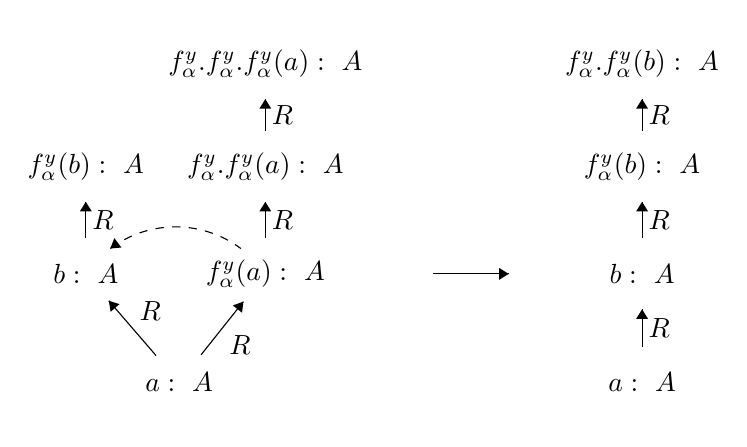
\begin{tikzpicture}[scale=0.15]
	\tikzstyle{every node}+=[inner sep=0pt]
	\draw [white] (11.7,-48.7) circle (3);
	\draw (11.7,-48.7) node {$a:\mbox{ }A$};
	\draw [white] (3.8,-39.5) circle (3);
	\draw (3.8,-39.5) node {$b:\mbox{ }A$};
	\draw [white] (19,-39.5) circle (3);
	\draw (19,-39.5) node {$f_\alpha^y(a):\mbox{ }A$};
	\draw [white] (50.9,-48.7) circle (3);
	\draw (50.9,-48.7) node {$a:\mbox{ }A$};
	\draw [white] (50.9,-39.5) circle (3);
	\draw (50.9,-39.5) node {$b:\mbox{ }A$};
	\draw [white] (30.2,-39.5) circle (3);
	\draw [white] (42.6,-39.5) circle (3);
	\draw [white] (19,-30.4) circle (3);
	\draw (19,-30.4) node {$f_\alpha^y.f_\alpha^y(a):\mbox{ }A$};
	\draw [white] (50.9,-30.4) circle (3);
	\draw (50.9,-30.4) node {$f_\alpha^y(b):\mbox{ }A$};
	\draw [white] (3.8,-30.4) circle (3);
	\draw (3.8,-30.4) node {$f_\alpha^y(b):\mbox{ }A$};
	\draw [white] (19,-21.7) circle (3);
	\draw (19,-21.7) node {$f_\alpha^y.f_\alpha^y.f_\alpha^y(a):\mbox{ }A$};
	\draw [white] (50.9,-21.7) circle (3);
	\draw (50.9,-21.7) node {$f_\alpha^y.f_\alpha^y(b):\mbox{ }A$};
	\draw [black] (9.75,-46.42) -- (5.75,-41.78);
	\fill [black] (5.75,-41.78) -- (5.9,-42.71) -- (6.65,-42.06);
	\draw (8.3,-42.65) node [right] {$R$};
	\draw [black] (13.56,-46.35) -- (17.14,-41.85);
	\fill [black] (17.14,-41.85) -- (16.25,-42.17) -- (17.03,-42.79);
	\draw (15.91,-45.52) node [right] {$R$};
	\draw [black,dashed] (5.874,-37.351) arc (126.72001:53.27999:9.242);
	\fill [black,dashed] (5.87,-37.35) -- (6.81,-37.27) -- (6.22,-36.47);
	\draw [black] (50.9,-45.7) -- (50.9,-42.5);
	\fill [black] (50.9,-42.5) -- (50.4,-43.3) -- (51.4,-43.3);
	\draw (51.4,-44.1) node [right] {$R$};
	\draw [black] (33.2,-39.5) -- (39.6,-39.5);
	\fill [black] (39.6,-39.5) -- (38.8,-39) -- (38.8,-40);
	\draw [black] (19,-36.5) -- (19,-33.4);
	\fill [black] (19,-33.4) -- (18.5,-34.2) -- (19.5,-34.2);
	\draw (19.5,-34.95) node [right] {$R$};
	\draw [black] (50.9,-36.5) -- (50.9,-33.4);
	\fill [black] (50.9,-33.4) -- (50.4,-34.2) -- (51.4,-34.2);
	\draw (51.4,-34.95) node [right] {$R$};
	\draw [black] (3.8,-36.5) -- (3.8,-33.4);
	\fill [black] (3.8,-33.4) -- (3.3,-34.2) -- (4.3,-34.2);
	\draw (4.3,-34.95) node [right] {$R$};
	\draw [black] (19,-27.4) -- (19,-24.7);
	\fill [black] (19,-24.7) -- (18.5,-25.5) -- (19.5,-25.5);
	\draw (19.5,-26.05) node [right] {$R$};
	\draw [black] (50.9,-27.4) -- (50.9,-24.7);
	\fill [black] (50.9,-24.7) -- (50.4,-25.5) -- (51.4,-25.5);
	\draw (51.4,-26.05) node [right] {$R$};
	\end{tikzpicture}
	\end{center}
	\caption{Atomic Merging Example}
	\label{figure:atomic-merging}
	\end{figure}

When $x$ is mergeable on $t$ in $F$, for each trigger $\tr=(\alpha,\sigma)$ applied on $F$ where the range of $\sigma$ is included in $\des(x)$, the trigger $h_{x/t}(\tr)= (\alpha,h_{x/t} \circ \sigma)$ has been or will be applied. Therefore, all the facts containing variables in $\des(x)$ are or will be redundant. But we do not want to supress all these facts because we know that if they are not yet in the facts that contain variables in $\des(t)$, they would be computed. Instead, we would like to ``recycle'' these facts. That is this intuition that leads us to define atomic merging. \todo{je ne suis pas convaincu par ce que j'ai écrit dans ce paragraphe }



For example, in the Figure \ref{figure:atomic-merging}, $f_\alpha^y(a)$ is mergeable on $b$ in the left factbase. The atomic merging of $f_\alpha^y(a)$ on $b$ in this factbase produces the right factbase. The following definition describes the operation that will replace the computation of the core in the core chase. We will show that for a chase derivation $D =F_0,...,F_k$ of $K$, if we apply our operation on $F_k$, then it computes the core of a factbase that could have been produced by continuing the derivation $D$.



\begin{definition}
For a factbase $F$, a \emph{merge} sequence of $F$ is a sequence $F_0,\ldots,F_n$ of factbases such that:
\begin{itemize}
\item $F_0 = F$.
\item For $i \in \{1,\ldots,n\}$, the factbase $F_i$ is the atomic merging of a variable $x$ on a term $t$ in $F_{i-1}$.
\item The factbase $F_n$ does not contain a mergeable variable.
\end{itemize}
Then, $\Merge(F) = F_n$.
\end{definition}

The result of the \Merge\ operation is unique up to isomorphism. 


\begin{figure}
\begin{center}
\begin{tikzpicture}[scale=0.2]
\tikzstyle{every node}+=[inner sep=0pt]
\draw [white] (8.2,-36.8) circle (3);
\draw (8.2,-36.8) node {$a:A$};
\draw [white] (4,-24.6) circle (3);
\draw (4,-24.6) node {$b:\mbox{ }C,D$};
\draw [white] (12.2,-24.6) circle (3);
\draw (12.2,-24.6) node {$f_\alpha^z(a):\mbox{ }C$};
\draw [white] (12.2,-11.2) circle (3);
\draw (12.2,-11.2) node {$f_\beta^z.f_\alpha^z(a):\mbox{ }E$};
\draw [white] (4,-11.2) circle (3);
\draw (4,-11.2) node {$c:\mbox{ }E$};
\draw [white] (15.5,-24.5) circle (3);
\draw [white] (31.1,-24.5) circle (3);
\draw [white] (33.4,-37.6) circle (3);
\draw (33.4,-37.6) node {$a:\mbox{ }A$};
\draw [white] (33.4,-23.8) circle (3);
\draw (33.4,-23.8) node {$b:\mbox{ }C,D$};
\draw [white] (29.3,-11.2) circle (3);
\draw (29.3,-11.2) node {$c:\mbox{ }E$};
\draw [white] (38.1,-11.2) circle (3);
\draw (38.1,-11.2) node {$f_\beta^z(b):\mbox{ }E$};
\draw [white] (35.8,-24.5) circle (3);
\draw [white] (50.5,-24.5) circle (3);
\draw [white] (54.6,-37.6) circle (3);
\draw (54.6,-37.6) node {$a:\mbox{ }A$};
\draw [white] (54.6,-24.5) circle (3);
\draw (54.6,-24.5) node {$b:\mbox{ }C,D$};
\draw [white] (54.6,-11.2) circle (3);
\draw (54.6,-11.2) node {$c:E$};
\draw [black] (7.22,-33.96) -- (4.98,-27.44);
\fill [black] (4.98,-27.44) -- (4.76,-28.36) -- (5.71,-28.03);
\draw (6.86,-29.97) node [right] {$S$};
\draw [black] (4,-21.6) -- (4,-14.2);
\fill [black] (4,-14.2) -- (3.5,-15) -- (4.5,-15);
\draw (4.5,-17.9) node [right] {$R$};
\draw [black] (9.13,-33.95) -- (11.27,-27.45);
\fill [black] (11.27,-27.45) -- (10.54,-28.06) -- (11.49,-28.37);
\draw (10.97,-31.39) node [right] {$S$};
\draw [black] (12.2,-21.6) -- (12.2,-14.2);
\fill [black] (12.2,-14.2) -- (11.7,-15) -- (12.7,-15);
\draw (12.7,-17.9) node [right] {$R$};
\draw [red] (18.5,-24.5) -- (28.1,-24.5);
\fill [red] (28.1,-24.5) -- (27.3,-24) -- (27.3,-25);
\draw [black] (33.4,-34.6) -- (33.4,-26.8);
\fill [black] (33.4,-26.8) -- (32.9,-27.6) -- (33.9,-27.6);
\draw (33.9,-30.7) node [right] {$S$};
\draw [black] (32.47,-20.95) -- (30.23,-14.05);
\fill [black] (30.23,-14.05) -- (30,-14.97) -- (30.95,-14.66);
\draw (32.12,-16.82) node [right] {$R$};
\draw [black] (34.45,-20.99) -- (37.05,-14.01);
\fill [black] (37.05,-14.01) -- (36.3,-14.59) -- (37.24,-14.94);
\draw (36.51,-18.31) node [right] {$R$};
\draw [red] (38.8,-24.5) -- (47.5,-24.5);
\fill [red] (47.5,-24.5) -- (46.7,-24) -- (46.7,-25);
\draw [black] (54.6,-34.6) -- (54.6,-27.5);
\fill [black] (54.6,-27.5) -- (54.1,-28.3) -- (55.1,-28.3);
\draw (55.1,-31.05) node [right] {$S$};
\draw [black] (54.6,-21.5) -- (54.6,-14.2);
\fill [black] (54.6,-14.2) -- (54.1,-15) -- (55.1,-15);
\draw (55.1,-17.85) node [right] {$R$};
\end{tikzpicture}
\end{center}
\caption{Merging Example}
\label{figure:merging}
\end{figure}


\begin{example} \label{example: merging}
In the Figure \ref{figure:merging}, we merge the factbase of the left. The variable $f_\alpha^z(a)$ is mergeable on $b$, an atomic merging of $f_\alpha^z(a)$ on $b$ yields the factbase of the middle. Now, $f_\beta^z(b)$ is mergeable on $c$, an atomic merging of $f_\beta^z(b)$ on $c$ produces the factbase of the right. The last factbase is the result of the merge since it does not contain any mergeable variable.

\end{example}



We can now consider two new chases:

\begin{definition}[derivation] \label{fairness}
A \emph{merge derivation} for a \ALCH\ knowledge base $K = (R,F)$ is a (possibly infinite) sequence $D = F_0, F_1, F_2, \ldots$ where $F_0 = F$, and for $i >0$, either $F_{i}= \Appl(F_{i-1},t_i)$ is obtained by an application with $t_i$ an oblivious trigger, or $F_i$ is obtained by the merging of $F_{i-1}$. $D$ is \emph{fair} if: 
\begin{itemize}
\item For every $i$, for every oblivious trigger $t$ applicable on $F_i$, there exists $k \leq i$ or $k > i$ such that $t$ is useless on $F_k$; or there exists $k > i$ such that $t$ is not anymore an oblivious trigger for $F_k$.
\item For every $i$, there exists $k \geq i$ such that $F_k$ is a core.
\end{itemize}

A \emph{merge chase} for a knowledge base $K= (R,F)$ is a fair atomic merge derivation (resp. a fair merge derivation) $D=F_0,F_1,F_2,\ldots$
\end{definition}

We also introduce the \emph{atomic merge chase} in order to simplify a futur proof, and to show that we can be more flexible on the use of the merge chase. The atomic merge chase is a merge chase where we use the atomic merge operation instead of the merge operation.   

\begin{definition}
The atomic merge chase (resp. the merge chase)  \emph{terminates} on $K$ if it is a finite derivation $D=F_0,F_1,F_2,\ldots,F_k$. We note, in this case, $\MC(K) = F_k$ the result of the merge chase.
\end{definition}

The result of the merge chase is unique up to isomorphism. The type $(\exists_+)$ is the only type of \ALCH\ rules that leads to the introduction of one existentially variable when we apply a rule of this type. Therefore:

\begin{proposition} \label{prec}
Consider a variable $t$ that occurs in a merge chase derivation $D$ of some \ALCH\ knowledge base $K$.
Then, $t$ is of the form $f^y_\alpha(u)$ where $u$ is a term, $\alpha$ is a rule of the form $(\exists_+)$ in $K$, and $y$ is the only existentially quantified variable occurring in $\alpha$.
Moreover, $u$ is the only term in $D$ such that $u \prec t$.
\end{proposition}




\begin{proposition} \label{partial_order}
For a factbase $F$ that occurs in a merge chase derivation of some \ALCH\ knowledge base, $\prec^+$ is a strict partial order over the set of terms of $F$.
\end{proposition}

\begin{proof}
Suppose for a contradiction that there exists a term $t$ such that $t \prec^+ t$. There exists then $n \in \N \setminus \{0\}$ and terms $t_0,\ldots,t_n$ such that $t=t_0 \prec t_1 \prec \cdots \prec t_n = t$. By Proposition \ref{prec}, there exists rules $\alpha_1,\ldots, \alpha_n$ and variables $v_1,\ldots,v_n$ such that $t_n = f_{\alpha_n}^{v_n}(f_{\alpha_{n-1}}^{v_{n-1}}(\cdots f_{\alpha_1}^{v_1}(t_0)\cdots))$. It is a contradiction since $t_0 = t$ and $t_n=t$. Therefore $\prec^+$ is irreflexive. By construction, $\prec^+$ is transitive; So $\prec^+$ is a strict partial order
\end{proof}

We have shown in the proof that the graph induced by $\prec$ does not contain any cycle. We obtain the following result from Propositions \ref{prec} and \ref{partial_order}:

\begin{proposition}
For a factbase $F$ that occurs in a merge chase derivation of some \ALCH\ knowledge base, the graph induced by $\prec$ is a forest of trees and the root of each tree is a constant.
\end{proposition}




%We can then associate the depth of a variable:
%
%\begin{definition}
%Let $F$ be a factbase that occurs in a core chase derivation of the knowledge base $K$. We define the \emph{depth} of a term $t$ by induction:
%\begin{itemize}
%\item 
%\end{itemize}
%\end{definition}






%Notice that the definition of siblings can be shorted because, due to the form of the \ALCH\ axioms, for a term $t$, there exists a unique term $t'$ and a unique binary relation $R$ such that $R(t',t)\in F$. So we can replace the last condition in the definition about the existence of $t$ by: there exists a term $t$ and a predicate $R$ such that $R(t,t_1) \in F$ and $R(t,t_2) \in F$. We write this more complex definition because it works in more general cases.

We define the notion of tree of a term $t$ that is all the facts containing only variables in $\des(t)$:

\begin{definition}[Tree]
For a term $t$ occurring in a chase derivation of the \ALCH\ knowledge base $K$, we pose:
\begin{align*}
	\Tree_{F}(t) = \{&A(u) \mid A(u) \in F \wedge u \in \des(t)\}~\cup \\
	\{&R(u,x) \mid R(u,x) \in F \wedge u,x \in \des(t)\}
\end{align*}
\end{definition}




We show that the atomic merge chase computes only universal models thanks to the two next propositions.

\begin{proposition} \label{step1}
	Let $D = F_0,F_1,\ldots,F_m$ be an atomic merge chase derivation of a knowledge base $K$
	and let $x$ be a variable mergeable on a term $t$ in $F_m$.
	Then, there exists an atomic merge chase derivation $D'$ of the form $D, E$ (where $E$ is a sequence of factbases) such that:
	\begin{enumerate}
	\item Consider some factbase $F \in E$ and its predecessor $G$ in $D'$.
	Then, there is an oblivious trigger $t = (\alpha, \sigma)$ for $G$ such that $F = \Appl(G, t)$.
	%\item $F_{m+1}= \Appl(F_m,t_m),\ldots,F_k = \Appl(F_{k-1},t_{k-1})$ have been obtained by a rule application, where $t_m,\ldots,t_{k-1}$ are oblivious triggers,
	\item The last element of $E$ is the factbase $F_m \cup h_{x/t}(\Tree_{F_m}(x))$. 
	\end{enumerate}
	\end{proposition}

We pose \emph{$\Fut(F_m,t,x) = F_m \cup h_{x/t}(\Tree_{F_m}(x))$}.
	
\begin{figure} 
\begin{center}
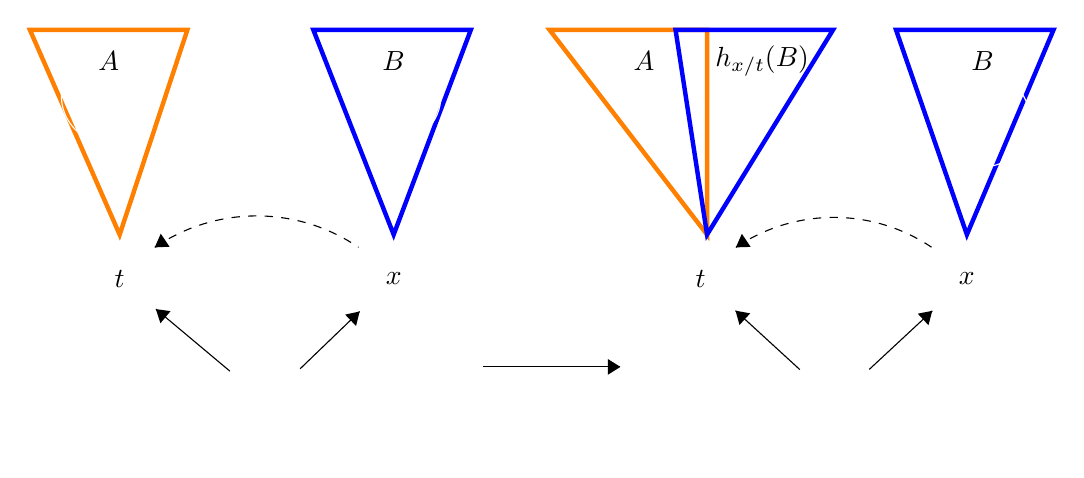
\begin{tikzpicture}[scale=0.2]
\tikzstyle{every node}+=[inner sep=0pt]
\draw [white] (20,-48.6) circle (3);
\draw [white] (10.7,-40.8) circle (3);
\draw (10.7,-40.8) node {$t$};
\draw[orange, ultra thick] (10.7,-38) -- (5,-25) -- (15,-25) -- cycle;
\draw [white] (28.1,-40.8) circle (3);
\draw (28.1,-40.8) node {$x$};
\draw[blue, ultra thick] (28.1,-38) -- (23,-25) -- (33,-25) -- cycle;
\draw [white] (10,-29.2) circle (3);
\draw (10,-27) node {$A$};
\draw [white] (28.1,-29.2) circle (3);
\draw (28.1,-27) node {$B$};
\draw [white] (56.1,-48.6) circle (3);
\draw [white] (47.6,-40.8) circle (3);
\draw (47.6,-40.8) node {$t$};
\draw[orange, ultra thick] (48,-38) -- (38,-25) -- (48,-25) -- cycle;
\draw[blue, ultra thick] (48,-38) -- (46,-25) -- (56,-25) -- cycle;
\draw [white] (64.5,-40.8) circle (3);
\draw (64.5,-40.8) node {$x$};
\draw[blue, ultra thick] (64.5,-38) -- (60,-25) -- (70,-25) -- cycle;
\draw (44,-27) node {$A$};
\draw (51.5,-27) node {$h_{x/t}(B)$};
\draw [white] (65.5,-30.7) circle (3);
\draw (65.5,-27) node {$B$};
\draw [white] (30.8,-46.4) circle (3);
\draw [white] (45.5,-46.4) circle (3);
\draw [black] (17.7,-46.67) -- (13,-42.73);
\fill [black] (13,-42.73) -- (13.29,-43.63) -- (13.93,-42.86);
\draw [black] (22.16,-46.52) -- (25.94,-42.88);
\fill [black] (25.94,-42.88) -- (25.02,-43.08) -- (25.71,-43.8);
\draw [black,dashed] (12.931,-38.807) arc (124.28182:55.71818:11.484);
\fill [black] (12.93,-38.81) -- (13.87,-38.77) -- (13.31,-37.94);
\draw [black] (53.89,-46.57) -- (49.81,-42.83);
\fill [black] (49.81,-42.83) -- (50.06,-43.74) -- (50.74,-43);
\draw [black] (58.3,-46.56) -- (62.3,-42.84);
\fill [black] (62.3,-42.84) -- (61.38,-43.02) -- (62.06,-43.75);
\draw [black,dashed] (49.831,-38.809) arc (124.01582:55.98418:11.116);
\fill [black] (49.83,-38.81) -- (50.77,-38.78) -- (50.21,-37.95);
\draw [black] (33.8,-46.4) -- (42.5,-46.4);
\fill [black] (42.5,-46.4) -- (41.7,-45.9) -- (41.7,-46.9);
\end{tikzpicture}
\end{center}

\caption{Illustration of the proof}
\label{proof}
\end{figure}

Graphically, in the Figure \ref{proof}, if we note $A=\Tree_{F_m}(t)$ and $B=\Tree_{F_m}(x)$, then we want do an atomic merge derivation from the left factbase to the right factbase.


To prove the Proposition \ref{step1}, we will look all the triggers dealing with the variables in $\des(x)$ and apply them on the variables in $\des(t)$ if the triggers have not already been applied.

\begin{proof}
In order to define an atomic merge chase sequence such as $D'$, we first introduce some sequences of oblivious triggers:
\begin{itemize}
\item Let $t_1 = (\alpha_1,\sigma_1),\ldots, t_n =(\alpha_n,\sigma_n)$ be the maximal sequence of oblivious triggers such that:
(1) for each $1 \leq i \leq n$, there is some $1 \leq j \leq m$ such that $\Appl(F_j, t_i) = F_{j+1}$;
(2) if $F_k = \Appl(F_{k-1}, t_i)$ and $F_l = \Appl(F_{l-1},t_j)$ for some $i, j \in \{1, \ldots, n\}$ and  some $1 \leq k < l \leq m$, then $i<j$; and (3) the range of $\sigma_i$ is a subset of $\des(x)$ for each $1 \leq i \leq n$.
\item Let $t'_1, \ldots, t'_o$ be the maximal subsequence of $(\alpha_1, h_{x/t} \circ \sigma_1), \ldots, (\alpha_n, h_{x/t} \circ \sigma_n)$ that are not useless triggers for $F_m$
\end{itemize}

$t'_1, \ldots, t'_o$ are the triggers that \todo{}

Let $F_{m+i} = \Appl(F_{m+i-1}, t'_i)$ for each $1 \leq i \leq o$.
We show via induction that the sequence $D' = D, F_{m+1}, \ldots, F_{m+o}$ satisfies conditions 1. and 2. stated in the proposition. 

Suppose for $1 \leq i \leq n$ that $D, F_{m+1}, \ldots, F_{m+i-1}$ is an atomic merge derivation such that the triggers $t_1',\ldots,t_{i-1}'$ are useless for $F_{m+i-1}$. There exists $1 \leq j \leq n$ such that the trigger $t_i'$ is equal to $h_{x/t}(t_j)$. The oblivious trigger $h_{x/t}(t_j)$ is not useless for $F_{m+i-1}$. Depending on the form of the rule $\alpha_j$, there exists five different cases:
	\begin{itemize}
	\item If $\alpha_j$ is of the form $A(u) \rightarrow \exists v.R(u,v) \wedge B(v)
	$. We have $A(\sigma_j(u)) \in F_m$.
		\begin{itemize}
		\item If $\sigma_j(u) = x$, then $A(x) \in F_m$. As $t$ is a strong sibling of $x$ in $F_m$, $A(t) \in F_m$. So $A(h_{x/t}(\sigma_j(u))) \in F_{m+i-1}$ since $h_{x/t}(\sigma_j(u)) = t$.  
		\item If $x \prec^+ \sigma_j(u)$, then the fact $A(\sigma_j(u)))$ is in $\sigma_k^s(Head(\alpha_k))$ where $k<j$. By induction hypothesis, $h_{x/t}(t_j)$ is useless for $F_{m+i-1}$ so  $A(h_{x/t}(\sigma_j(u)))\in F_{m+i-1}$. 
		\end{itemize}
Therefore $h_{x/t}(t_j)$ is an oblivious trigger for $F_{m+r(i-1)}$.
\todo{j'ai pas eu le temps de modifier les autres cas mais ils sont presque pareil}
	\item If $\alpha_j$ is of the form $A_1(u) \wedge A_2(u) \rightarrow B(u)$. We have $A_1(\sigma_j(u)),A_2(\sigma_j(u)) \in F_m$.
		\begin{itemize}
		\item If $\sigma_j(u) = x$, then $A_1(x),A_2(x) \in F_m$. As $t$ is a strong sibling of $x$ in $F_m$, we have $A_1(t),A_2(t) \in F_m$. So $A_1(h_{x/t}(\sigma_j(u))),A_2(h_{x/t}(\sigma_j(u))) \in F_{m+r(i-1)}$ since $h_{x/t}(\sigma_j(u)) = t$.  
		\item If $x \prec^+ \sigma_j(u)$, then the facts $A_1(\sigma_j(u)))$ and $A_2(\sigma_j(u)))$ are in $\sigma_j^s(Head(\alpha_j))$ where $j<i$. We have then $A_1(h_{x/t}(\sigma_j(u))),A_2(h_{x/t}(\sigma_j(u)))\in B_{i-1}'$ so by induction hypothesis, $A_1(h_{x/t}(\sigma_j(u))),A_2(h_{x/t}(\sigma_j(u)))\in F_{m+r(i-1)}$. 
		\end{itemize}
Therefore $h_{x/t}(t_j)$ is an oblivious trigger for $F_{m+r(i-1)}$.  

\item If $\alpha_j$ is of the form $A(u) \wedge R(u,v) \rightarrow B(v)$.
	\begin{itemize}
		\item If $\sigma_j(u) = x$, then $A(x) \in F_m$. As $t$ is a strong sibling of $x$ in $F_m$, $A(t)\in F_m$. Thus $A(h_{x/t}(\sigma_j(u))) \in F_{m+r(i-1)}$.
		\item If $x \prec^+ \sigma_j(u)$, then the fact $A(\sigma_j(u)))$ is in $\sigma_j^s(Head(\alpha_j))$ where $j<i$. We have then $A(h_{x/t}(\sigma_j(u)))\in B_{i-1}'$ so by induction hypothesis, $A(h_{x/t}(\sigma_j(u)))\in F_{m+r(i-1)}$. 
		\end{itemize}
The fact $R(\sigma_j(u),\sigma_j(v))$ is in $\sigma_j^s(Head(\alpha_j))$ where $j<i$. We have then $R(h_{x/t}(\sigma_j(u)),h_{x/t}(\sigma_j(v)))\in B_{i-1}'$ so by induction hypothesis, $R(h_{x/t}(\sigma_j(u)),h_{x/t}(\sigma_j(v)))\in F_{m+r(i-1)}$. 		

Therefore, the facts $A(h_{x/t}(\sigma_j(x)))$ and $R(h_{x/t}(\sigma_j(u)),h_{x/t}(\sigma_j(v)))$ are in $ F_{m+r(i-1)}$. Thus $h_{x/t}(t_j)$ is an oblivious trigger for $F_{m+r(i-1)}$.
\item If $\alpha_j$ is of the form $R(u,v) \wedge B(v) \rightarrow A(u)$. $\sigma_j(u) \neq x$ since $A(t) \in F_{m}$

The facts $R(\sigma_j(u),\sigma_j(v)),B(\sigma_j(v))$ have been introduced by oblivious triggers in $\{tr_1,\ldots,tr_{i-1}\}$. So, by induction hypothesis, the facts $R(h_{x/t}(\sigma_j(u)),h_{x/t}(\sigma_j(v)))$ and $B(h_{x/t}(\sigma_j(v)))$ are in $ F_{m+r(i-1)}$. Therefore $h_{x/t}(t_j)$ is an oblivious trigger for $F_{m+r(i-1)}$.
\item If $\alpha_j$ is of the form $R_1(u,v) \wedge R_2(u,v) \rightarrow S(u,v)$.

The facts $R_1(\sigma_j(u),\sigma_j(v)),R_2(\sigma_j(u),\sigma_j(v))$ are in $\sigma_j^s(Head(\alpha_j))$ where $j<i$. We have then $R_1(h_{x/t}(\sigma_j(u)),h_{x/t}(\sigma_j(v))),R_2(h_{x/t}(\sigma_j(u)),h_{x/t}(\sigma_j(v)))\in B_{i-1}'$ so by induction hypothesis, $R_1(h_{x/t}(\sigma_j(u)),h_{x/t}(\sigma_j(v))),R_2(h_{x/t}(\sigma_j(u)),h_{x/t}(\sigma_j(v)))\in F_{m+r(i-1)}$. 



	\end{itemize} 

As $h_{x/t}(t_j)$ is an oblivious trigger for $F_{m+i-1}$, $D_i$ is an atomic merge derivation. By definition of an application, we have $h_{x/t} \circ \sigma_j^s(Head(\alpha_j)) \subseteq F_{m+r(i)}$ and so $B_i' = B_{i-1} \cup h_{x/t} \circ \sigma_j^s(Head(\alpha_j)) 	\subseteq F_{m+i}$.
Therefore, $H(i)$ is true.


We have proved the heredity. So, $D_n$ is the oblivious derivation that we was looking for. We have $F_{m+k} = F_m \cup h_{x/t}(\Tree_{F_m}(x))$.

\end{proof}




\begin{proposition} \label{step2}
Let $D = F_0,F_1,\ldots,F_m$ be an atomic merge chase derivation for the knowledge base $K$. Assume that $x$ is mergeable on $t$ in $F_m$, the atomic merging of $x$ on $t$ in $F_m$ is a retract of $\Fut(F_m,t,x)$ .
\end{proposition}

\begin{proof}
The atomic merging of $x$ on $t$ in $F_m$ is $h_{x/t}(F_m)$. By the Proposition \ref{step1}, $\Fut(F_m,t,x)= F_m \cup h_{x/t}(\Tree_{F_m}(x))$. So, $h_{x/t}(F_m) \subseteq \Fut(F_m,t,x) $ since $\Fut(F_m,t,x) = \Tree_{F_m}(x) \cup h_{x/t}(F_m)$. Finally, as $h_{x/t}(\Fut(F_m,t,x)) = h_{x/t}(F_m)$, we have that $h_{x/t}(F_m) \vDash \Fut(F_m,t,x)$.
\end{proof}

The following theorem is a corollary of Propositions \ref{step1} and \ref{step2}:

\begin{theorem} \label{universality atomic merge}
Let $D = F_0,F_1,\ldots$ be an atomic merge chase derivation for the knowledge base $K$. The factbases $F_0,F_1,\ldots$ are universal for $K$.
\end{theorem}

\begin{proof}
We prove the proposition by induction. By definition of a model, $M \vDash F_0$ so the initial step is true.
Suppose that $M \vDash F_{n-1}$, where $n >0$, and that $F_{n-1}$ is not the last factbase of the derivation $D$.
\begin{itemize}
\item If $F_n=\Appl(F_{n-1},t)$, where $t=(\alpha,\sigma)$ is an oblivious trigger, by Proposition \ref{universality-application}, $M \vDash F_n$.



\item If $F_n$ is the atomic merging of a variable $x$ on a term $t$ in $F_{n-1}$, then according to Proposition \ref{step1}, there exists factbases $G_0,\ldots,G_k$ such that (1) $G_0 = F_{n-1}$, (2) $G_k = \Fut(F_{n-1},t,x)$, and (3) for $0 \leq i \leq k-1$, $G_{i+1} =\Appl(G_i,t)$ where $t$ is an oblivious trigger for $G_i$. We have then by direct induction on $0 \leq i \leq k$ and by Proposition \ref{universality-application}, $M \vDash G_i$. Therefore $M \vDash \Fut(F_{n-1},t,x)$, so $M$ is a model of the atomic merging of $x$ on $t$ in $F_{n-1}$ (that is $F_n$) since, by Proposition \ref{step2}, $F_n$ is a subset of $\Fut(F_{n-1},t,x)$.
\end{itemize}
\end{proof}




The main reason to prefer the merge chase instead of the atomic merge chase is that unless the atomic merging operations are applied exhaustively, the merge chase may not terminate on inputs that admit finite universal models:


\begin{theorem} \label{necessity of atomic merge}
There exists a \ALCH\ knowledge base and an infinite atomic merge chase derivation for $K$ such that $K$ admits a finite universal model.
\end{theorem}

\begin{figure}
\begin{center}
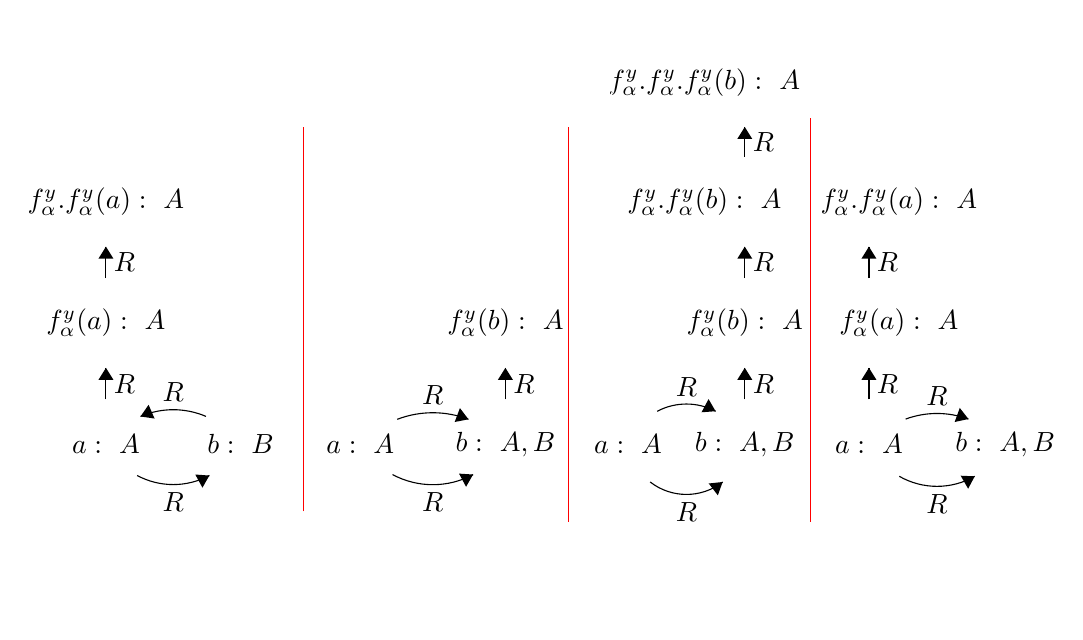
\begin{tikzpicture}[scale=0.19]
\tikzstyle{every node}+=[inner sep=0pt]
\draw [white] (16,-25.6) circle (3);
\draw (16,-25.6) node {$b:\mbox{ }B$};
\draw [white] (7,-25.6) circle (3);
\draw (7,-25.6) node {$a:\mbox{ }A$};
\draw [white] (7,-17.5) circle (3);
\draw (7,-17.5) node {$f_\alpha^y(a):\mbox{ }A$};
\draw [white] (7,-9.4) circle (3);
\draw (7,-9.4) node {$f_\alpha^y.f_\alpha^y(a):\mbox{ }A$};
\draw [white] (24,-25.6) circle (3);
\draw (24,-25.6) node {$a:\mbox{ }A$};
\draw [white] (33.7,-25.6) circle (3);
\draw (33.7,-25.6) node {$b:\mbox{ }A,B$};
\draw [white] (41.9,-25.6) circle (3);
\draw (41.9,-25.6) node {$a:\mbox{ }A$};
\draw [white] (49.7,-25.6) circle (3);
\draw (49.7,-25.6) node {$b:\mbox{ }A,B$};
\draw [white] (58,-25.6) circle (3);
\draw (58,-25.6) node {$a:\mbox{ }A$};
\draw [white] (67.1,-25.6) circle (3);
\draw (67.1,-25.6) node {$b:\mbox{ }A,B$};
\draw [white] (33.7,-17.5) circle (3);
\draw (33.7,-17.5) node {$f_\alpha^y(b):\mbox{ }A$};
\draw [white] (49.7,-17.5) circle (3);
\draw (49.7,-17.5) node {$f_\alpha^y(b):\mbox{ }A$};
\draw [white] (49.7,-9.4) circle (3);
\draw (47,-9.4) node {$f_\alpha^y.f_\alpha^y(b):\mbox{ }A$};
\draw [white] (49.7,-1.4) circle (3);
\draw (47,-1.4) node {$f_\alpha^y.f_\alpha^y.f_\alpha^y(b):\mbox{ }A$};
\draw [white] (58,-17.5) circle (3);
\draw (60,-17.5) node {$f_\alpha^y(a):\mbox{ }A$};
\draw [white] (58,-9.4) circle (3);
\draw (60,-9.4) node {$f_\alpha^y.f_\alpha^y(a):\mbox{ }A$};
\draw [white] (20.2,-33.1) circle (3);
\draw [white] (20.2,-1.4) circle (3);
\draw [white] (37.9,-33.8) circle (3);
\draw [white] (37.9,-1.4) circle (3);
\draw [white] (54.1,-33.8) circle (3);
\draw [white] (54.1,-0.8) circle (3);
\draw [black] (13.913,-27.695) arc (-61.74408:-118.25592:5.098);
\fill [black] (13.91,-27.7) -- (12.97,-27.63) -- (13.45,-28.51);
\draw (11.5,-28.8) node [below] {$R$};
\draw [black] (9.313,-23.747) arc (113.21358:66.78642:5.549);
\fill [black] (9.31,-23.75) -- (10.25,-23.89) -- (9.85,-22.97);
\draw (11.5,-22.8) node [above] {$R$};
\draw [black] (31.542,-27.634) arc (-61.78869:-118.21131:5.695);
\fill [black] (31.54,-27.63) -- (30.6,-27.57) -- (31.07,-28.45);
\draw (28.85,-28.81) node [below] {$R$};
\draw [black] (48.224,-28.129) arc (-52.06714:-127.93286:3.943);
\fill [black] (48.22,-28.13) -- (47.29,-28.23) -- (47.9,-29.02);
\draw (45.8,-29.46) node [below] {$R$};
\draw [black] (65.072,-27.751) arc (-60.23294:-119.76706:5.079);
\fill [black] (65.07,-27.75) -- (64.13,-27.71) -- (64.63,-28.58);
\draw (62.55,-28.92) node [below] {$R$};
\draw [black] (26.469,-23.941) arc (110.98089:69.01911:6.65);
\fill [black] (31.23,-23.94) -- (30.66,-23.19) -- (30.31,-24.12);
\draw (28.85,-23) node [above] {$R$};
\draw [black] (43.847,-23.403) arc (117.88071:62.11929:4.176);
\fill [black] (47.75,-23.4) -- (47.28,-22.59) -- (46.81,-23.47);
\draw (45.8,-22.42) node [above] {$R$};
\draw [black] (60.451,-23.924) arc (110.20979:69.79021:6.075);
\fill [black] (64.65,-23.92) -- (64.07,-23.18) -- (63.73,-24.12);
\draw (62.55,-23.05) node [above] {$R$};
\draw [black] (7,-22.6) -- (7,-20.5);
\fill [black] (7,-20.5) -- (6.5,-21.3) -- (7.5,-21.3);
\draw (7.5,-21.55) node [right] {$R$};
\draw [black] (7,-14.5) -- (7,-12.4);
\fill [black] (7,-12.4) -- (6.5,-13.2) -- (7.5,-13.2);
\draw (7.5,-13.45) node [right] {$R$};
\draw [black] (33.7,-22.6) -- (33.7,-20.5);
\fill [black] (33.7,-20.5) -- (33.2,-21.3) -- (34.2,-21.3);
\draw (34.2,-21.55) node [right] {$R$};
\draw [black] (49.7,-22.6) -- (49.7,-20.5);
\fill [black] (49.7,-20.5) -- (49.2,-21.3) -- (50.2,-21.3);
\draw (50.2,-21.55) node [right] {$R$};
\draw [black] (49.7,-14.5) -- (49.7,-12.4);
\fill [black] (49.7,-12.4) -- (49.2,-13.2) -- (50.2,-13.2);
\draw (50.2,-13.45) node [right] {$R$};
\draw [black] (49.7,-6.4) -- (49.7,-4.4);
\fill [black] (49.7,-4.4) -- (49.2,-5.2) -- (50.2,-5.2);
\draw (50.2,-5.4) node [right] {$R$};
\draw [black] (58,-22.6) -- (58,-20.5);
\fill [black] (58,-20.5) -- (57.5,-21.3) -- (58.5,-21.3);
\draw (58.5,-21.55) node [right] {$R$};
\draw [black] (58,-14.5) -- (58,-12.4);
\fill [black] (58,-12.4) -- (57.5,-13.2) -- (58.5,-13.2);
\draw (58.5,-13.45) node [right] {$R$};
\draw [red] (37.9,-30.8) -- (37.9,-4.4);

\draw [red] (20.2,-30.1) -- (20.2,-4.4);

\draw [red] (54.1,-30.8) -- (54.1,-3.8);

\end{tikzpicture}
\end{center}

\caption{Example where the atomic merge chase is not efficient}
\label{figure:atomic merge chase not efficient}
\end{figure}


\begin{proof} 
Let $F= \{R(a,b),R(b,a),A(a),A(b)\}$ and $R = \{\alpha = A(x) \rightarrow \exists y.R(x,y) \wedge A(y), \beta = B(x) \rightarrow A(x)\}$. We consider for the knowledge base $K=(R,F)$, the atomic merge chase derivation  $F_0 =F,F_1,F_2,...$
\begin{itemize}

\item We applied to $F_0$ the oblivious trigger $t_1 = (\alpha, \{x \mapsto a\})$;
\item we then applied to $F_1$, the oblivious trigger $t_2 = (\alpha, \{x \mapsto f_\alpha^y(a)\})$ giving rise to the first factbase of the Figure \ref{figure:atomic merge chase not efficient};
\item we then apply the oblivious trigger $t_3 = (\beta, \{x \mapsto b\})$ to obtain the factbase $F_3$;
\item At this moment, $f_\alpha^y(a)$ is mergeable on $b$ so we do an atomic merging of $f_\alpha^y(a)$ on $b$ to get $F_4$ that is the second factbase of the figure;
\item $F_5$ is obtained by the application of the oblivious trigger $t_4 = (\alpha, \{x \mapsto f_\alpha^y(b)\})$ and $F_6$ by the oblivious trigger $t_5 = (\alpha, \{x \mapsto f_\alpha^y(f_\alpha^y(b))\})$, $F_6$ is the third factbase of the figure;
\item At this moment, $f_\alpha^y(b)$ is mergeable on $a$ so we do an atomic merging of $f_\alpha^y(b)$ on $a$ to get $F_7$ that is the last factbase of the figure; 
\item We can repeat this infinitely. 

\end{itemize} 
 But $K$ admits a finite universal model: $U = F \cup \{B(b)\}$. 

\todo{Improve write-up; discuss. is it better ?}



\end{proof}



We want now prove that a merging computes a core:

\begin{proposition} \label{core}
For a factbase $G$ that occurs in a merge chase derivation of some \ALCH\ knowledge base, $\Merge(G)$ is a core.
\end{proposition}

\begin{proof}
%\item The $\mathcal{ALCH}$-pruning algorithm only take off facts of the factbase. Consequently, $\textit{prune}(G) \subseteq G$.
%\item We consider the homorphism $h:G \to \textit{prune}(G)$ created during the $\mathcal{ALCH}$-pruning algorithm. For $x \in \Vars(G)$, suppose that $h(x) \neq x$. According to the $\mathcal{ALCH}$-pruning algorithm, $x$ has been erased \todo{à préciser}. So $x \notin \Vars(\textit{prune}(G))$. So ${h}_{|\textit{Prune}(G)}=id_{|\textit{Prune}(G)}$. We have shown that $h$ is a retract so $\textit{prune}(G)$ is a retract of $G$.
Suppose for a contradiction that $\Merge(G)$ is not a core. There exists a factbase $G' \subsetneq \Merge(G)$ such that $G'$ is a retract of $\Merge(G)$. By Proposition \ref{retract}, there exists then a retractation $h$ from $\Merge(G)$ to $G'$. We have $var(\Merge(G))\setminus var(G') \neq \emptyset$. Let $x$ be a $\prec$-minimal variable of this set. The term $x$ is a variable, so has been introduced by the chase due to a rule of the form $(\exists_+)$, so there exists a term $t$ such that $t \prec x$. 
\begin{itemize}
\item We have $\Preds^2_{\Merge(G)}(t,x) \neq \emptyset$. By $\prec$-minimality of $x$, $t \in \Vars(G')$. So, as $h$ is a retractation: $h(t) = t$, so for $R \in \Preds^2_{\Merge(G)}(t,x)$, $h(R(t,x)) = R(t,h(x)) \in \Merge(G)$ and so $R \in \Preds^2_{\Merge(G)}(t,h(x))$. Thus $\Preds^2_{\Merge(G)}(t,x) \subseteq \Preds^2_{\Merge(G)}(t,h(x))$.
\item As $\Preds^2_{\Merge(G)}(t,x) \subseteq \Preds^2_{\Merge(G)}(t,h(x))$ and $\Preds^2_{\Merge(G)}(t,x) \neq \emptyset$, we have $t \prec h(x)$.
\item $x \notin G'$ and $h(x) \in G'$ so $h(x) \neq x$. 
\item Let $A \in \Preds^1_{\Merge(G)}(x)$. $h(A(x)) \in \Merge(G)$ so $A(h(x)) \in \Merge(G)$ so $\Preds^1_{\Merge(G)}(x) \subseteq \Preds^1_{\Merge(G)}(h(x))$. 
\end{itemize}
Consequently, $x$ is mergeable on $h(x)$ in $\Merge(G)$ which results on a contradiction. Hence, $\Merge(G)$ is a core.
\end{proof}	

$\Merge(G)$ is a core but not necessarily the core of $G$. We need the following lemma to prove that the merge chase computes an universal model:

\begin{proposition} \label{lemme}
	Let $D=F_0,\ldots,F_k, \ldots$ be an atomic merge chase derivation of a knowledge base $K$, $\alpha$ be a rule, and $\sigma$ be a substitution such that $\sigma(\textit{Body}(\alpha)) \subseteq F_k$. There exists then $n \geq 0$ and a substitution $\hat \sigma$ prolonging $\sigma$ such that for all $j \geq n$, $\hat \sigma(\textit{Head}(\alpha)) \subseteq F_j$.\todo{Potential error: discuss.} 
\end{proposition}

\begin{proof}
	As the derivation $D$ is fair, there exists $n \geq 0$ such that $\Appl(F_n,t) = F_n$; thus $\sigma^s(\textit{Head}(\alpha)) \subseteq F_n$.
	We show by induction that for $n\leq j $, there exists a substitution $\hat \sigma$ prolonging $\sigma$ such that $\hat \sigma(\textit{Head}(\alpha)) \subseteq F_j$. The initialisation is true with $\hat \sigma = \sigma^s$. Assume that there exists a substitution $\hat \sigma$ prolonging $\sigma$ such that $\hat \sigma(\textit{Head}(\alpha)) \subseteq F_{j-1}$ where $n < j$. If $F_j = \Appl(F_{j-1},t)$ where $t$ is an oblivious trigger, then $\hat \sigma(\textit{Head}(\alpha)) \subseteq F_{j}$ since $F_{j-1} \subseteq F_j$. If $F_j$ is the atomic merging of the variable $x$ on the term $t$ in $F_{j-1}$, then $F_j = h_{x/t}(F_{j-1})$. Therefore $h_{x/t}(\hat \sigma(\textit{Head}(\alpha))) \subseteq F_j$ and so $h_{x/t} \circ \hat \sigma$ is the substitution that we are looking for. The heredity is proved.
\end{proof}


%\begin{definition}
%$\tr = (\alpha,\sigma, \hat \sigma)$ is a \emph{stupid trigger} if $(\alpha,\sigma)$ is an oblivious trigger, and if $\hat \sigma$ extends $\sigma$ and is defined on $\Vars(\textit{Head}(\alpha))$. The factbase $\Appl(F,\tr)=F \cup \hat \sigma(\textit{Head}(\alpha))$ is called an \emph{application} on the factbase $F$ through the stupid trigger $\tr = (\alpha,\sigma, \hat \sigma)$. A \emph{stupid derivation} from a knowledge base $K= (F,R)$ is a (possibly infinite) sequence $D=F_0,tr_1,F_1,tr_2,F_2,\ldots$ where $(F_i)_{i \in \N}$ are factbases, $tr_i$ are stupid triggers, $F_0 = F$, and for $i >0$, $F_{i}= \Appl(F_{i-1},tr_i)$ is obtained by an application. The stupid derivation $D=F_0,F_1,F_2,\ldots$ is \emph{fair} if for every $i$ and every stupid trigger $\tr = (\alpha,\sigma, \hat \sigma)$ applicable on $F_i$, there exists $k \geq i$ such that there exists a stupid trigger $\tr' = (\alpha,\sigma, \hat \sigma')$ that verified $\Appl(F_{k},\tr') = F_k$. A \emph{stupid chase} for a knowledge base $K= (F,R)$ is a fair stupid derivation $D=F_0,tr_1,F_1,tr_2,F_2,\ldots$ $F_0 \subseteq F_1 \subseteq F_2 \subseteq \ldots$ so we can pose \emph{$\textit{Stp(K)}$} = $\cup_{i \in \N}F_i$.
%We say that the stupid chase \emph{terminates} if $\textit{Stp(K)}$ is finite.
%\end{definition}




\begin{proposition} \label{finite <- terminates}
The merge chase computes a finite universal model of $K$ when it terminates.
\end{proposition}

\begin{proof}
Let $D = F_0,\ldots,F_n$ be a merge chase for $K =(R,G)$. 
\begin{itemize}
\item The merge chase never take off ground facts and $G =F_0$ so $G \subseteq F_n$. We have then $F_n \vDash G$. Suppose that there exists a rule $\alpha$ in $R$ and a substitution $\sigma$ such that $F_n \vDash \sigma(\textit{Body}(\alpha))$. Then by Proposition \ref{lemme}, there exists a substitution $\hat \sigma$ prolonging $\sigma$ such that $\hat \sigma(\textit{Head}(\alpha)) \subseteq F_n$. We can conclude that $F_n \vDash R$, so $F_n$ is a model of $K$.
\item According to Proposition \ref{universality atomic merge}, $F_n$ is a universal model of $K$.
\item $F_n$ is finite.
\end{itemize}
\end{proof}

\begin{proposition} \label{finite -> terminates}
If there exists a finite universal model for a \ALCH\ knowledge base $K = (R,F)$, then the merge chase terminates.
\end{proposition}

\begin{proof}
\begin{itemize}
\item Suppose for a contradiction that $K$ admits a finite universal model $U$ for $K$ and does not admit a finite merge chase sequence. There exists so an infinite merge chase sequence $D= F_0, F_1, \ldots$
\item A term $t$ is \emph{redundant} with respect to this sequence if $t \in \Terms(F_i)$ and $t \notin \Terms(F_j)$ for some $i < j$.
\item For each $i$, let $G_i$ be the maximal subset of $F_i$ that does not contain redundant terms.

\item We pose $M = \cup_i~G_i$. For a model $N$ of $K$ and for $i \in \N$, there exists a homomorphism $h_i$ from $F_i$ to $N$ since $F_i$ is universal for $K$ by Proposition \ref{universality atomic merge}. As $G_i \subseteq F_i$, $h_i$ is a homomorphism from $G_i$ to $N$. Finally, $\cup_i~h_i$ is a homomorphism from $M$ to $N$ so $M$ is universal for $K$.

\item Constants cannot be redondants\todo{redundant}, so $F \subseteq M$ since $G_0 =F$. We have then $M \vDash F$. Suppose that there exists a rule $\alpha$ in $R$ and a substitution $\sigma$ such that $M \vDash \sigma(\textit{Body}(\alpha))$. There exists then $n \geq 0$ such that $G_n \vDash \sigma(\textit{Body}(\alpha))$ so $F_n \vDash \sigma(\textit{Body}(\alpha))$ since $G_n \subseteq F_n$. Then by Proposition \ref{lemme}, for $k \geq n$, there exists a substitution $\sigma_k$ prolonging $\sigma$ such that $\sigma_k(\textit{Head}(\alpha)) \subseteq F_k$. If $\alpha$ is not of the form $(\exists_+)$, then $\sigma_k = \sigma$. As all the variables in the range of $\sigma$ are in $\Vars(M)$, they are not redundant and so $\sigma(\textit{Head}(\alpha)) \subseteq G_n \subseteq M$. Otherwise $\alpha$ is of the form $A(x) \rightarrow \exists y.R(x,y) \wedge B(y)$. We have then $\sigma_k = \sigma \cup \{y \mapsto f_\beta^y(\sigma(x))\}$ with $\beta$ a rule in $R$. There is a finite number of rules in $R$ and once a variable is merged, it does not reappear, therefore there exists $k \geq n$ such that for all $i \geq k$, $\sigma_i = \sigma_k$.Then $\sigma_k(y)$ is not redundant and as all the variables in the range of $\sigma$ are in $\Vars(M)$, they are not redundant, so $\sigma_k(\textit{Head}(\alpha)) \subseteq G_k \subseteq M$. We can conclude that $M \vDash R$, so $M$ is an universal model of $K$.\todo{Discuss this point.}


\item As $M$ is an universal model of $K$, $M \vDash U$. There exists then a homomorphism $h$ from $U$ to $M$. As $U$ is finite, the factbase $h(U)\subseteq M$ is also finite. The sequence $G_0,G_1,\ldots$ is monotonic (that is $G_0 \subseteq G_1 \subseteq \cdots$) so there exist $i$ such that $h(U) \subseteq G_i$. We have then $F_i \vDash h(U)$ since $G_i \subseteq F_i$. We have $h(U) \vDash U$, so $F_i\vDash U$. 

\item As $D$ is fair, there exists $j \geq i$ such that $F_j$ is a core. 
%We have $F_k \subseteq F_i$ so all the triggers for $F_k$ has been applied in the derivation $F_0,F_1,\ldots,F_k$.

\item By proposition \ref{universality atomic merge}, $F_j$ is universal for $K$ so $U \vDash F_j$. We have $F_j \vDash U$ since $F_j \vDash F_i$, so $F_j$ is isomorphe\todo{Isomorphic.} to the core of $U$. Therefore $F_j$ is an universal model for $K$.

\item There exists a finite number of triggers for $F_j$ and $D$ is fair. So, there exists $k \geq j$ such that all the triggers for $F_j$ has been applied in the derivation $F_0,F_1,\ldots,F_k$. Note that this step is necessary to garantee the first condition in the Definition \ref{fairness} of fairness.

\item As $D$ is fair, there exists $l\geq k$ such that $F_l$ is a core. As $F_j$ is a model for $K$, $F_l = F_j$.  
%We have $F_k \subseteq F_i$ so all the triggers for $F_k$ has been applied in the derivation $F_0,F_1,\ldots,F_k$.



\item The derivation $F_0,\ldots,F_l$ is then fair so it is a finite merge chase sequence that leads us to a contradiction.
\end{itemize}
\end{proof}

The following theorem is then a direct consequence of Propositions \ref{finite <- terminates} and \ref{finite -> terminates}.

\begin{theorem}
The merge chase computes an universal model if and only if there exists an universal model.
\end{theorem}

We will now describe a deterministic algorithm to merge a factbase:

\begin{definition}[Merging]
Let $F$ be a factbase that occurs in a merge chase derivation of the knowledge base $K$.

\begin{algorithm}[H] \label{algo}
\SetAlgoLined


    Let $\textbf{\Vars}(F) = \{x_1,\ldots, x_n\}$ be such that $(x_i \prec^+ x_j) \Rightarrow i < j$ \;
    \For{$i =1 \text{ to } n$}{
    	\If{$x_i$ is still a variable in $F$}{
			\For{all term $t$ such that $x_i$ is mergeable on $t$}{
				$F \leftarrow$ the atomic merging of $x_i$ on $t$ in $F$.
			}
		}
	}
return $F$
\caption{Merge($F$):}


\end{algorithm}
At line 1, we can sort terms like that because, by proposition \ref{partial_order}, $\prec^+$ is a strict partial order over the set of variables of $F$.
\end{definition}



Note that the application of an atomic merge may result in new mergeable variables. Therefore, we have to be carefull about the order of the variables in the Algorithm \ref{algo}. In the Example \ref{example: merging}, if we treat $f_\beta^z(f_\alpha^z(a))$ before $f_\alpha^z(a)$, then at the moment where we treat $f_\beta^z(f_\alpha^z(a))$, it does not have any term $t$ yet such that $f_\beta^z(f_\alpha^z(a))$ is mergeable on $t$. At the end, we get the factbase of the middle and we will not have merged every possible mergeable variable.


The Example \ref{necessity of atomic merge} shows the importance of doing a total merging. We have to prove that our merging algorithm does a total merging:

\begin{proposition}\label{no_more_siblings}
Let $G$ be a factbase that occurs in a chase derivation of the knowledge base $K$. There does not exists a term $t$ and a variable $x$ such that $x$ is mergeable on $t$ in $\Merge(G)$\todo{I would name this differently to indicate that you are referencing Algorithm 1 and not the declarative definition that was discussed before.}.
\end{proposition}

\begin{proof} 
Suppose for a contradiction that there exists a term $t$ and a variable $x$ such that $x$ is mergeable on $t$ in $\Merge(G)$, that is, there exists a term $t'$ such that $\Preds^2_{\Merge(G)}(t',x) \neq \emptyset$ and $\Preds_{\Merge(G)}^2(t',x) \subseteq \Preds_{\Merge(G)}^2(t',t)$. This case can happen only if $x$ became mergeable after that $x$ has been traited by the merging algorithm. Thus, during the merging, there has been an atomic merging on $t'$. Let $y$ be the variable merged on $t'$ such that $y \prec x$. We note $G^1$ the factbase just before the atomic merging of $y$ on $t'$ and we note $G^2$ the factbase just after the atomic merging. There exists a term $t_0$ such that $\Preds^2_{G^1}(t_0,y) \neq \emptyset$ and $\Preds_{G^1}^2(t_0,y) \subseteq \Preds_{G^1}^2(t_0,t')$. The factbase $G^1$ is in the left of the Figure \ref{figure:proof} and the factbase $G^2$ is in the right (we do not represent all the graphs):

\begin{figure}
\begin{center}
\begin{tikzpicture}[scale=0.2]
\tikzstyle{every node}+=[inner sep=0pt]
%\filldraw[color=red!60, fill=red!5, very thick](17,-38) circle (6);
%\filldraw[color=red!60, fill=red!5, very thick](60,-39) circle (6);
%\filldraw[color=red!60, fill=red!5, very thick](10,-11) circle (4);
%\filldraw[color=red!60, fill=red!5, very thick](25,-11) circle (4);
%\filldraw[color=red!60, fill=red!5, very thick](65,-11) circle (4);
%\filldraw[color=red!60, fill=red!5, very thick](54,-11) circle (4);
\draw [white] (17.1,-35.9) circle (3);
\draw (17.1,-35.9) node {$t_0$};
\draw [white] (10.1,-24.1) circle (3);
\draw (10.1,-24.1) node {$t'$};
\draw [white] (24.1,-24.1) circle (3);
\draw (24.1,-24.1) node {$y$};
\draw [white] (24.1,-12.4) circle (3);
\draw (24.1,-12.4) node {$x$};
\draw [white] (10.1,-12.4) circle (3);
\draw (10.1,-12.4) node {$t$};
\draw [white] (30.7,-24.6) circle (3);
\draw [white] (50.4,-24.6) circle (3);
\draw [white] (59.7,-36.8) circle (3);
\draw (59.7,-36.8) node {$t_0$};
\draw [white] (59.7,-25.3) circle (3);
\draw (59.7,-25.3) node {$t'$};
\draw [white] (53.4,-13.2) circle (3);
\draw (53.4,-13.2) node {$t$};
\draw [white] (65.4,-13.2) circle (3);
\draw (65.4,-13.2) node {$x$};
\draw [black] (15.57,-33.32) -- (11.63,-26.68);
\fill [black] (11.63,-26.68) -- (11.61,-27.62) -- (12.47,-27.11);

\draw [black] (10.1,-21.1) -- (10.1,-15.4);
\fill [black] (10.1,-15.4) -- (9.6,-16.2) -- (10.6,-16.2);

\draw [black] (18.63,-33.32) -- (22.57,-26.68);
\fill [black] (22.57,-26.68) -- (21.73,-27.11) -- (22.59,-27.62);

\draw [black] (24.1,-21.1) -- (24.1,-15.4);
\fill [black] (24.1,-15.4) -- (23.6,-16.2) -- (24.6,-16.2);

\draw [black] (33.7,-24.6) -- (47.4,-24.6);
\fill [black] (47.4,-24.6) -- (46.6,-24.1) -- (46.6,-25.1);
\draw [black] (59.7,-33.8) -- (59.7,-28.3);
\fill [black] (59.7,-28.3) -- (59.2,-29.1) -- (60.2,-29.1);

\draw [black] (58.31,-22.64) -- (54.79,-15.86);
\fill [black] (54.79,-15.86) -- (54.71,-16.8) -- (55.6,-16.34);

\draw [black] (60.98,-22.59) -- (64.12,-15.91);
\fill [black] (64.12,-15.91) -- (63.33,-16.42) -- (64.23,-16.85);

\end{tikzpicture}
\end{center}

\caption{Illustration of the proof}
\label{figure:proof}
\end{figure}

We have $t_0 \prec t' \prec t$ and $t_0 \prec y \prec x$ so $x$ should have been treated by the algorithm after the merging of $t'$ and $y$ so the algorithm will merge $x$ on $t$. It is a contradiction. 
\end{proof}


\section{Conclusion}

\todo{Reiterate achievements briefly.}
\todo{Discuss future work: $\mathcal{ALCHI}$.}

\bibliographystyle{plain}
\bibliography{sample}


\end{document}

\subsection{\ALCHI}

\begin{definition}[\ALCHI\ axioms]
A \emph{\ALCHI\ axiom} is either a \ALCH\ axiom or an existential rule of the form:
\begin{align}
R_1(x,y) \wedge R_2(x,y) \rightarrow S(y,x)
\end{align}

A \emph{\ALCHI\ knowledge base} $K = (R,F)$ is a knowledge base where $R$ is a set of \ALCHI\ axioms and $F$ contains only predicates of arity one or two. 

\end{definition}

We have to modify the merge chase because it does not work anymore:

We keep the same relation $\prec$. It is still a strict partial order over the set of variables.